\documentclass[conference]{IEEEtran}
\IEEEoverridecommandlockouts
% The preceding line is only needed to identify funding in the first footnote. If that is unneeded, please comment it out.
\usepackage{cite}
\usepackage{array}
\usepackage{listings}
\usepackage{amsmath,amssymb,amsfonts}
\usepackage{algorithmic}
\usepackage{hyperref}
\usepackage{graphicx}
\usepackage{textcomp}
\usepackage{xcolor}
\def\BibTeX{{\rm B\kern-.05em{\sc i\kern-.025em b}\kern-.08em
    T\kern-.1667em\lower.7ex\hbox{E}\kern-.125emX}}
\begin{document}

\title{STMT\\
{\footnotesize \textsuperscript{}Six Things Must TODO\\
Break manerism by Ivy Lee method}}

\author{\IEEEauthorblockN{Changhoi Kim}
\IEEEauthorblockA{\textit{Dept. of Information System} \\
\textit{Hanyang Univ}\\
Seoul, Korea \\
changhoi0522@hanyang.ac.kr }
\and
\IEEEauthorblockN{Jungeun Kim}
\IEEEauthorblockA{\textit{Dept. of Information System} \\
\textit{Hanyang Univ}\\
Seoul, Korea \\
wjddms04@hanyang.ac.kr }
\and
\IEEEauthorblockN{Eunchai Kim}
\IEEEauthorblockA{\textit{Dept. of Information System} \\
\textit{Hanyang Univ}\\
Seoul, Korea \\
eunchai512@naver.com }
}

\maketitle

\begin{abstract}
STMT is an application that helps people practice Ivy Lee Method, a way to get rid of mannerisms and manage time efficiently. We use artificial intelligence speaker NUGU to help users set up 6 things each day and manage tasks to be done every day.
\end{abstract}
\begin{IEEEkeywords}
ivy lee method,  6 things, mannerism, nugu, ai speaker, todo list
\end{IEEEkeywords}

\begin{table}
\caption{Role Assignments}
\begin{center}
\begin{tabular}{ | m{5em} | m{2cm}| m{4cm} | }
\hline
\textbf{\textit{Role}}& \textbf{\textit{Name}}& \textbf{\textit{Task}} \\
\hline
User& NUGU Speaker and Application user & Application can use for free on iOS and AOS. Every NUGU Speaker and application users can use default feature of application. \\
\hline\
Customer& SKT and Application User & Customer want to solve the problems at an acceptable cost . SKT want application which is running on NUGU speaker, so more NUGU users get advantages. Application users who want more advanced feature of application will pay subscription fee. \\
\hline
Software Developer & Changhoi Kim, Jungeun Kim & Engineers create actual product. They demand core function requirements, which give then up to their developing process, to manager. Software developers’ goal is to satisfy users and customers by realizing close to the requirements. \\
\hline
Development Manager & Eunchai Kim & Development managers intercommunicate with Customer and Software developer to satisfy with whole stakeholders. They schedule timeline to stick to the project before deadline. They also build overall developing process and support software developers.\\
\hline
\end{tabular}
\label{tab1}
\end{center}
\end{table}

\section{Introduction}
Ivy Lee Method is a technology for efficient time management used over a long period of time. It is proposed by Ivy Lee to executives and employees to eliminate corporate manners and improve productivity. Next are the following the five steps:\\

\begin{enumerate}
\item Set up six things to do for next day before bed. \\
\item Arrange in the order of priority among the six things. \\
\item The things are executed according to the priority set, and the next thing cannot be carried out until the previous thing is completed. \\
\item If the assignment is not completed, the remaining tasks will be carried out the next day. \\
\item Repeat the above method every day. \\
\end{enumerate}
 
This method makes modern people, surrounded with many tasks, think of the most important ones to be carried out. Since the method is simple enough for anybody to follow, it can be implemented until the execution stage. Also to eliminate the fear of starting from scratch. Furthermore, this helps break down mannerism and create a productive day. \\
 
The most complete application derived from the existing Ivy Lee Method was the application called “6 things”. This application is a To-Do list app that writes down six things to do. However, it does not force a priority, but rather only writes down six To-Do list. Also it does not store the degree of achievement of other days. Moreover, record cannot be checked, feedbacks cannot be made and no retrospection. \\

STMT sends an alarm so that people can set the day or the next day task. Also sets the To-Do list and checks the list of achievement through the AI speaker NUGU. Using NUGU, people can also check the next thing to be completed or task that was completed. Through subscription services, we provide a dashboard to store daily records and check weekly and monthly attainment rates.\\

\section{Requirements}

\subsection{Mobile Application}

Mobile applications will be used by users. Both Android and iOS are available. Cross Platform applications to communicate with the server is required. There will be five four functions(login, task list, dashboard, social) in the application.\\

\begin{enumerate}
    \item Login: Users only use social login. So there are no local application login form. And there are no sign-up screen because the application will use the information which is from social login. There will be only simple login screen.
    \begin{enumerate}
        \item Additional information screen: Social login might give email and unique app id value. But if user refuses to provide an email and the user is new client, the user should type email manually for using application.\\
    \end{enumerate}
    \item Navigation tab: The Application has some features, so it need the navigation bar for split the domain. It is on the bottom of the screen.\\
    \item Tasks (Main Screen): Six tasks screen will be on the main screen. In addition to the task designation, various works will be available.
    \begin{enumerate}
        \item One task component: There is task component which shows the detail of one task.
        \begin{enumerate}
            \item Read tasks detail: By default, the component shows the detail of one task. it has "when", "where", "with whom" fields, and simple to-do list to complete the task.
            \item Set details of task: In this component, user can make detail of the task. The detail fields are as mentioned above.
            \item Update to-do status in a task: Each to-do in the to-do list of a task can be completed. When all the to-dos are completed, the task is completed, too. However if there are no detail to-do, user can complete the task by other button in detail component or in list component. \\
        \end{enumerate}
        \item Task list component: There is task list component which has plural task components.
        \begin{enumerate}
            \item Read task list of specific date: In this screen, the component shows the list of tasks. It is default screen of task list component.
            \item Add task: In task list screen, user can add task for next day (or next session of task list). The added task is consist of task component.
            \item Start tasks and lock the list: When user click lock button, the list become uneditable except complete the task. Lock time is set by user in settings screen.
            \item Check ongoing task and complete the task: When the task list is locked, user can find what task should be handled, and check the task as complete. If the task has specific to-do list, and user check the task as complete, all to-dos in the task is also checked as complete.
            \item Pass the remain incomplete tasks to next task list: When the session (user-set lock time) is over, and the list has remain tasks, The remaining list goes into the next (session's) task list.\\
        \end{enumerate}
        \item Dashboard: User can check the usage of the application in this component. There are graph for visualizing monthly, weekly, daily task processing degree. And also check the list of the specific date.\\
    \end{enumerate}
    
    \item Social: Users can find their own ranks on the list. The list shows the ranking of the users' friends or the world ranking, which is a ranking of every user who uses our app. It can add new friends to the list and share users' results of six tasks to the others. Also, search for other users and look for their result is available. \\
    \item Settings: User can set the option of the application. They can adjust alarm, Task list session time (Lock time), and change their account information in this component.\\

\end{enumerate}

\subsection{NUGU Service}

Also, user can access the application through NUGU AI speaker. User speak specific command and the NUGU speaker response and process the command. \\

\begin{enumerate}
    \item Check the ongoing task: User can complete the task which is currently in progress. \\
    \item Check the detailed task: User can check the detailed to-do list inside the ongoing task. \\
    \item Complete the task: User can complete the ongoing task. \\
    \item Check the remain tasks: User can check the remain tasks in the list.\\

\end{enumerate}

\section{Development Environment}


\subsection{Choice of software development platform}

\begin{enumerate}
    \item Which platform and why \\
    Our service operates mainly on mobile applications. We use Cross Platform application that is available for both Android and iOS operating systems and we develop app focusing on the latest version due to development environmental limitations and time constraints. We are using React Native since it can develop both platforms. Our app is an app service based, not the web, because it needs to have easy access to the tasks and provide alarm service to the specific ones. \\
    
    The server application will work on Linux based Lambda of AWS. DynamoDB on AWS will be used for database. Lambda and DynamoDB can save the cost while building simple applications because of its generous free tier. \\
    
    We do not have to worry about infrastructure and can focus on server application logic when we use managed services of AWS like DynamoDB and Lambda. In addition, we think that golang is a suitable language to operate in Lambda system since it remains simple executable binary after compilation and does not have to run virtual machine like JVM.\\
    
    \item Which programming language and why
    \begin{enumerate}
        \item Typescript \\
        Typescript, Javascript's superset, provides more stable development environment. By defining the interface and types, errors caused by misusing the type are prevented in advance. It can also easily identify the specific way of using methods and functions. In addition to the above advantages, it is freely available to use the large open source system of JavaScript.\\
        \item Go \\
        Go language is a compile language, that has fast performance as C language. There is no complicated grammar, and by unifying some of the code styles, it reduces the concern about the convention. By using the computing power efficiently, relatively little computing resources are required to achieve the same goal as other languages.\\
        
        \item Finally, both languages are growing rapidly in terms of language utilization, especially typescript is becoming the standard for JS development environments. Golang also has a huge growing community and is in line with recent technology trends.\\
    \end{enumerate}
    \item Provide a cost estimation for your built \\
    
    \begin{table}[h!]
    \caption{Cost estimation}
    \begin{center}
    \begin{tabular}{ | m{6cm} | m{2cm} | }
    \hline
    \textbf{\textit{Name of software / hardware}}& \textbf{\textit{Cost}} \\
    \hline
    Apple Developer Program & 129,000 won \\
    \hline\
    AWS Lambda & 0 dollar \\
    \hline
    AWS DynamoDB & 0 - 5 dollar \\
    \hline
    \end{tabular}
    \label{tab1}
    \end{center}
    \end{table}
    \item Provide clear information of your development environment
    \begin{itemize}
        \item MacOS Catalina 10.15.7
        \begin{itemize}
            \item 2.3 GHz 8 Core intel Core i9 
            \item 32GB 2667 MHz DDR4 Memory 
        \end{itemize}
        \item Windows 10
        \begin{itemize}
            \item 1.80 GHz 8 Core Intel i7
            \item 8GB Memory
        \end{itemize}
        \item Visual Studio Code 1.50.1
        \item Goland 11.0.8 (2020.2)
        \item Go 1.15
        \item Gin 1.6.3
        \item Node 12.18.3
        \item Typescript 4.0.3
        \item React Native 0.63.3
        \item Git 2.28.0 
        \item Other open sources
            \begin{itemize}
                \item \href{https://github.com/6-things-must-to-do/app/blob/develop/package.json}{\textbf{Link: Open source used in mobile application}}
                \item \href{https://github.com/6-things-must-to-do/backend/blob/develop/go.mod}{\textbf{Link: Open source used in the server}}
            \end{itemize}
    \end{itemize}
    \item Using any commercial cloud platform \\
    
    AWS Lambda and DynamoDB will be used to launch production servers.  Computing and Database resources are the same information written above, and AWS API Gateway service will be used to proxy HTTP requests to Lambda. \\
    
\end{enumerate}




\subsection{Software in use}
\begin{enumerate}
    \item Git \\
    Git is a distributed version-control system for tracking changes in source code during software development. It manage the code version and make co-working with other programmer more easier. There is branch system which is core of co-working in git-managed source code with many engineer. Each developer write code for different features and then, the codes can be merged easily by git. \\
    
    \item Github \\
    GitHub is an American multinational corporation that provides hosting for software development and version control using Git. It has features about git and also has own feature about source access control. Source code can be managed by permission in github. \\
    
    \item Golang and Gin \\
    Golang is a statically typed, compiled programming language designed at Google. Golang is known as fast as C and maintainable as JAVA. It is compilable language and when it is compiled, a single binary file is created. The binary file can excutable in various platform (Go build command has OS option which is about what platform the binary will be excuted in). \\
    Gin is go web framework. It's full name is gin-gonic. It helps engineer to build web application server easily. It is opensource and maintained by many contributers. \\
    
    \item AWS \\
    AWS stands for amazon web service, which provides cloud computer. AWS has many availability zone, so engineer can build safe and solid application. AWS provides various computing type, and there are many managed services. Managed service means that engineers do not have to concern about infrastructure. AWS ensures that the service logic will work. That services like Lambda, DynamoDB, etc is called AWS serverless services that make developer to focus to build application, not infratructure. \\
    
    \item Typescript \\
    Typescript is superset of javascript. Javascript is not type-safety language, so using javascript in huge project can make dangerous bug. Typescript can be used in javascript project, and also only typescript project. It is opensource and has huge engineer commnunity and maintained by Microsoft. \\
    
    \item React Native \\
    React Native is framework for mobile cross platform. This framework is created by Facebook. It works on Typescript and Javascript environment. TS/JS code create Native code which is written in JAVA (Android) and Objective-C(iOS).
    
\end{enumerate}

\subsection{Task distribution}

\begin{table}[h!]
\caption{Task distribution}
\begin{center}
\begin{tabular}{ | m{2cm} | m{6cm} | }
\hline
\textbf{\textit{Name}}& \textbf{\textit{Task Distribution}} \\
\hline
Changhoi Kim& Build servers, including databases, and manage the whole project (Server, DB) \\
\hline\
Jungeun Kim & Connect the server and the mobile app, and the data values received from the server (Redux, Container) \\
\hline
Eunchai Kim & Align the received data and design UI and CSS (Screen) \\
\hline
\end{tabular}
\label{tab1}
\end{center}
\end{table}

Our roles were distributed by technology rather than by app function. Our app has multiple functions, and we tried to divide the roles by the functions (ex. Making tasks/ Managing tasks/ Adding friends). However, we found out this method is inefficient, and it would be difficult to complete the project if we proceed it this way. It is because we realized that it is almost impossible to learn all the different skills to create a single function in time. Therefore, we eventually decided to divide the tasks by component of the app rather than the function, and let each person take charge of it. \\

\section{Specifications}
\subsection{Mobile Application}

\begin{figure}[htp] \centering 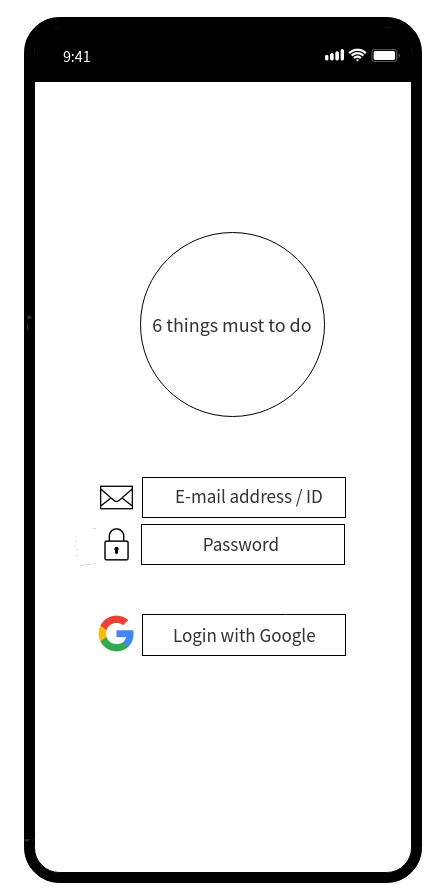
\includegraphics[width=200pt]{mockup_login} \caption{Login Screen} \label{fig:login} \end{figure}

\begin{enumerate}
    \item Login: \\
    Our application only has Google login. There are no other processes for signing up or signing in. Social login provides email, and unique app Id, etc. Using this information, application gets token from api server, and saves it in the device local storage. In the server, it takes social account information and gets user data in DynamoDB or creates user, then JWT which is to be used when user accesses api service.
    \begin{lstlisting}[frame=single]
    # in Application
    socialAccount := googlaLogin()
    token := getToken(socialAccount)
    saveTokenInLocalStorage(token)
    \end{lstlisting}
    
    \begin{lstlisting}[frame=single]
    # in API Server
    socialData := getRequest()
    user := getUserOrCreate(socialData)
    token := issueToken(user)
    response(token)
    \end{lstlisting}
 
\begin{figure}[htp] \centering 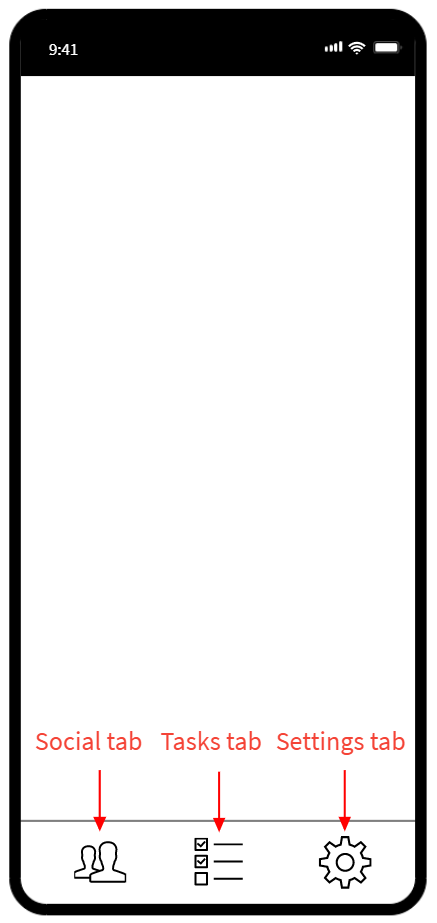
\includegraphics[width=200pt]{2) Navigation bar.PNG} \caption{Navigation tab} \label{fig:Navigation tab} \end{figure}
   
    \item Navigation tab: \\ 
    Navigation tab on the bottom of the screen includes social, tasks, settings tabs and is provided by open source named React Navigation. There is no other Network I/O.
    \begin{lstlisting}[frame=single]
    onChangeTab(targetScreen) {
        currentScreen = targetScreen
        re-render()
    }
    \end{lstlisting}
    
\begin{figure}[htp] \centering 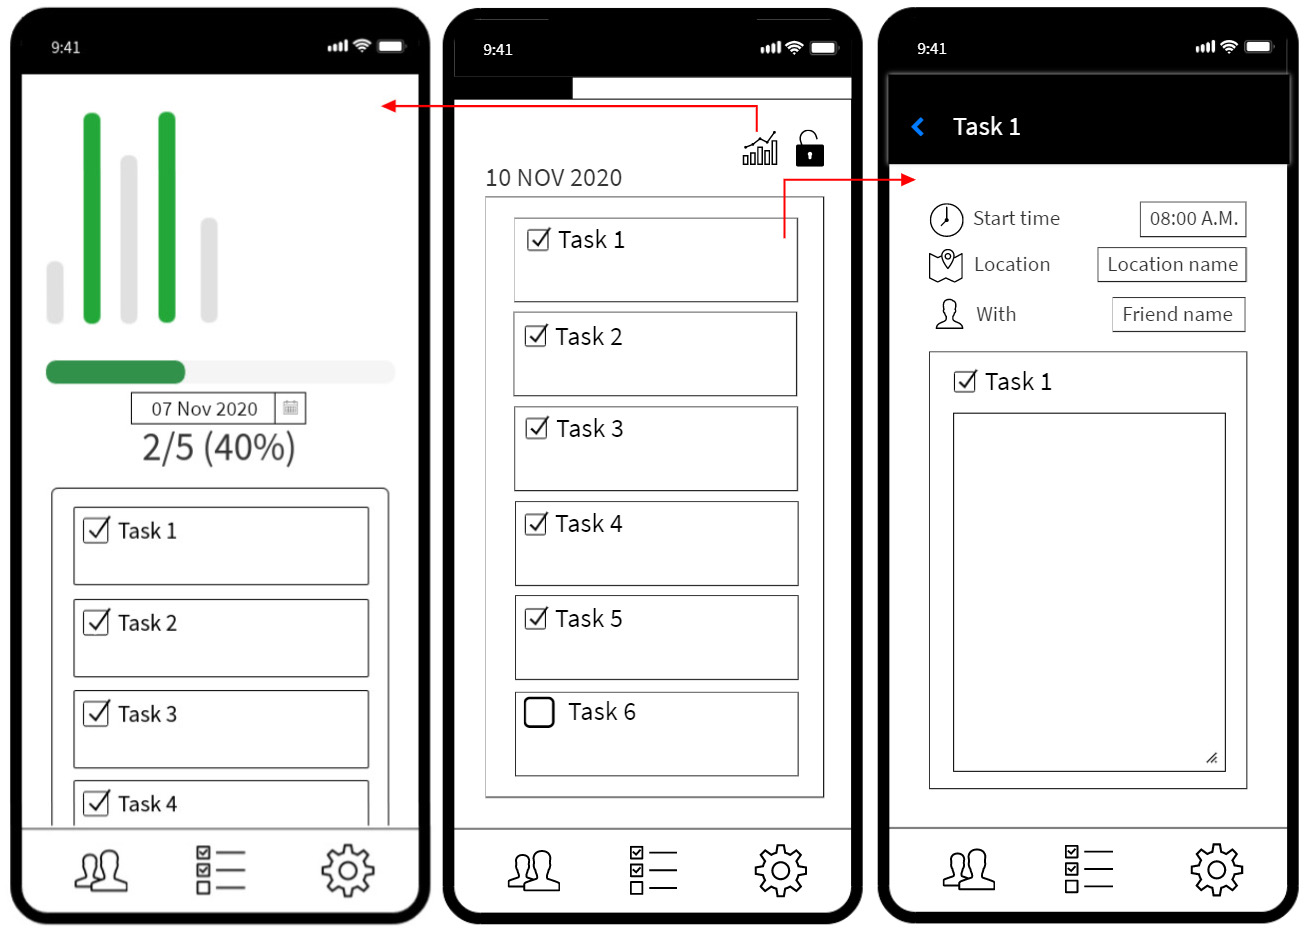
\includegraphics[width=270pt]{3) Tasks.jpg} \caption{Tasks (Main Screen)} \label{fig:Tasks} \end{figure}  
    
    \item Tasks (Main Screen): \\
    In main screen, authentication is required. Token should be stored in local storage and be used when calling API server service. User can click on the chart button to see their dashboard. Lock button on the right is a button to freeze the tasks and user can adjust the lock time in the settings. Details can be set when the user presses the tasks.
    \begin{enumerate}
        \item One task component: \\
        In a task component, there are details of a specific task. For showing the detail, API call is required. And in application, there is global store for saving data state. All the data is stored in one global Redux store, and it is only updated by dispatch function.
    \begin{lstlisting}[frame=single]
    # in Application
    data := apiCall(type, taskID)
    # CRUD API call
    dispatch(updateStore(data))
        .then(re-render())
    \end{lstlisting}
    
    \begin{lstlisting}[frame=single]
    # in API server
    type, taskID := request
    taskTable(where id = taskID)
        .action(type)
    # CRUD of task detail
    \end{lstlisting}
        \item Task list component: \\
        Task list component data is also managed by Redux store. All the API call and the result are being updated to the store through redux's dispatch function like above.

        \item Dashboard: \\
        The application should be able to get the log of user's usage by period. Data is stored in DynamoDB, so API call is required. And also the data is managed by redux.
    \begin{lstlisting}[frame=single]
    # in Application
    data := getLogOf["weekly"]()
    dispatch(updateDashboard(data))
        .then(re-render())
    \end{lstlisting}
\end{enumerate}
    
\begin{figure}[htp] \centering 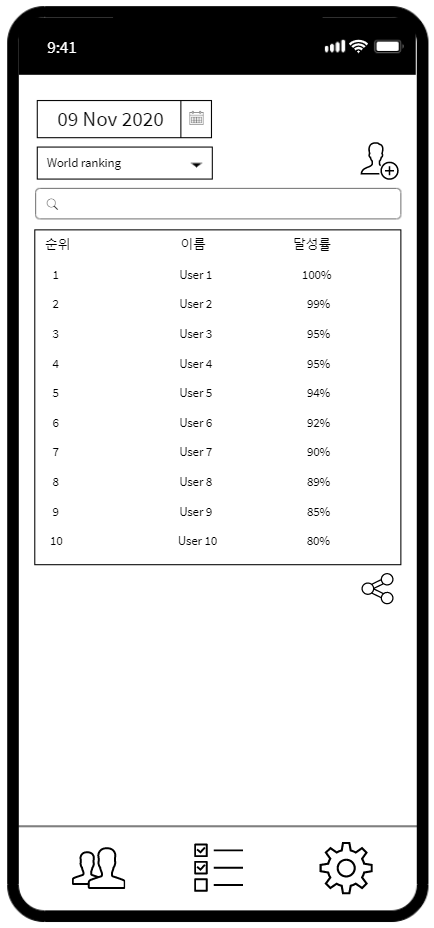
\includegraphics[width=200pt]{4) Social.PNG} \caption{Social} \label{fig:Social} \end{figure}
    
    \item Social: \\
    Friend list comes out when the user clicks the bottom social navigation tab. It shows the list of user's friends and at the same time, the ranking. Users can select to see the ranking of their friends or the world by pressing the ranking button. They can also add friends through the add button, and share the result through the share button. It is available to search the specific user, be friends and check the result of their six tasks.
    
\begin{figure}[htp] \centering 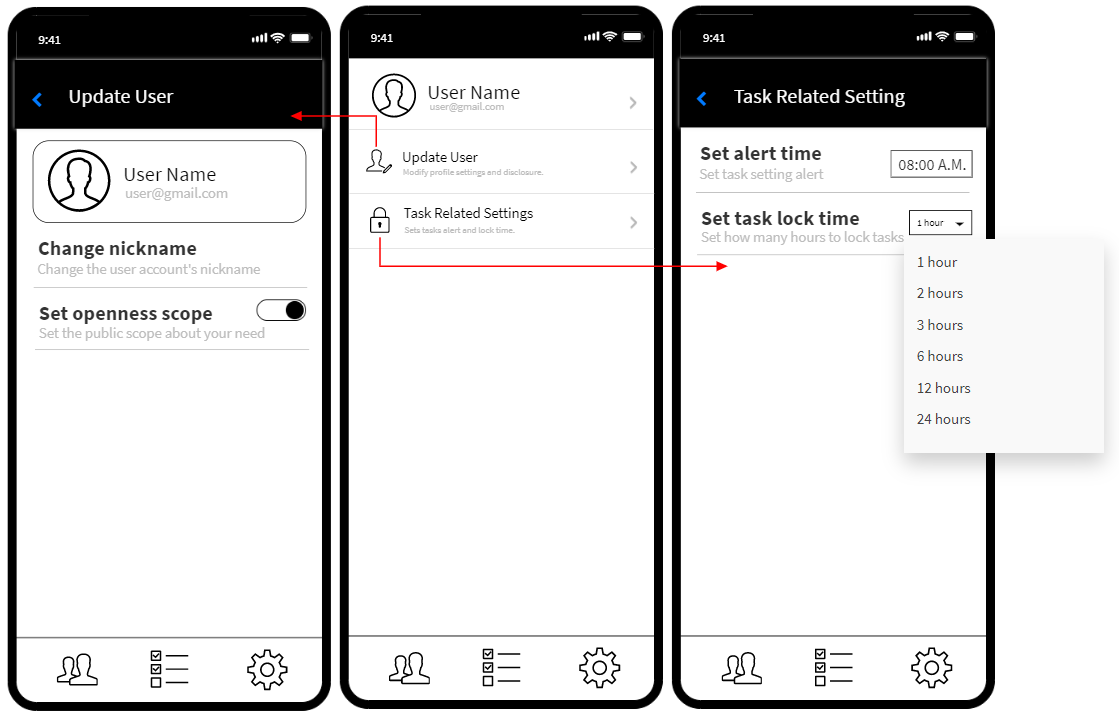
\includegraphics[width=260pt]{5) Settings.PNG} \caption{Settings} \label{fig:Settings} \end{figure}    
    
    \item Settings: \\
    In the settings screen, there are features about updating user information, and setting task related settings. Task related settings use local device's options. Alarm and task session time use device's timer API and updating user information uses API call.\\ \\ \\ \\
    \begin{lstlisting}[frame=single]
    # lock session time
    default = 8 * HOUR
    lockSessionTime = default
    onUpdateSessionTime((time) => {
        lockSessionTime = time
    }})
    
    # alarm
    default = 3 * HOUR
    triggerTimer = default
    onUpdateTriggerTime((time) => {
        triggerTimer = time
    })
    
    # update user info
    apiCall(updateData)
    \end{lstlisting}

\end{enumerate}

\subsection{NUGU Service}

User can use our application more conveniently by using the NUGU speaker. They can give instructions to the NUGU and it will respond to the user by doing a specific action. Following are the instructions that users can give to the speaker: Check ongoing task, Complete the task, Cancel the task, Check the remain task.\\

Every utterance command is sent to processing backend server through NUGU SDK. NUGU SDK processes the voice to string. And backend proxy server changes the string to valid command form and send it to the api server.

\begin{lstlisting}[frame=single]
voice > NUGU SDK > Processed voice string
> Backend Proxy server > API Server
\end{lstlisting}

\begin{table}[h]
\caption{NUGU Service Flow}
\begin{center}
\begin{tabular}{ | m{1cm} | m{8cm} | }
\hline
\textbf{\textit{Speaker}}& \textbf{\textit{Utterance}} \\
\hline
User & Aria, (trigger), tell me the ongoing task. \\
\hline\
NUGU & You are currently on task number [TaskNumber], and the task is [TaskDescription]. \\
\hline
User & Aria, (trigger), let me check the details. \\
\hline 
NUGU & Your task [NextTaskDescription], has the following details : [TaskToDoList]. \\
\hline
User & Aria, (trigger), let me complete the task. \\
\hline
NUGU & Your task number [TaskNumber] is completed, and the next task is [NextTaskDescription]. \\
\hline
User & Aria, (trigger), let me check the remain task. \\
\hline
NUGU & [RemainTasksNumber] more tasks to go. Next task is task number [TaskNumber], and it is [TaskDescription]. (And the next task is task number [TaskNumber], and it is [TaskDescription].) #Utterance repeats depends on the number of the remain tasks. \\
\hline
\end{tabular}
\label{tab1}
\end{center}
\end{table}

\begin{enumerate}
    \item Check ongoing task: \\
    User can look up which task they are on and the name of it. 
    
    \item Check the detailed task: \\
    User can check the detailed task. NUGU responds to-do list inside the ongoing task to the user.
    
    \item Complete the task: \\
    Task will be completed when the user completes the task by the speaker.
    
    \item Check the remain tasks: \\
    NUGU tells the user how many tasks are left and explains what number the next task is and what it is. \\
    
\end{enumerate}

\section{Architecture Design & Implementation}
\subsection{Overall architecture} 

\begin{figure}[htp] \centering 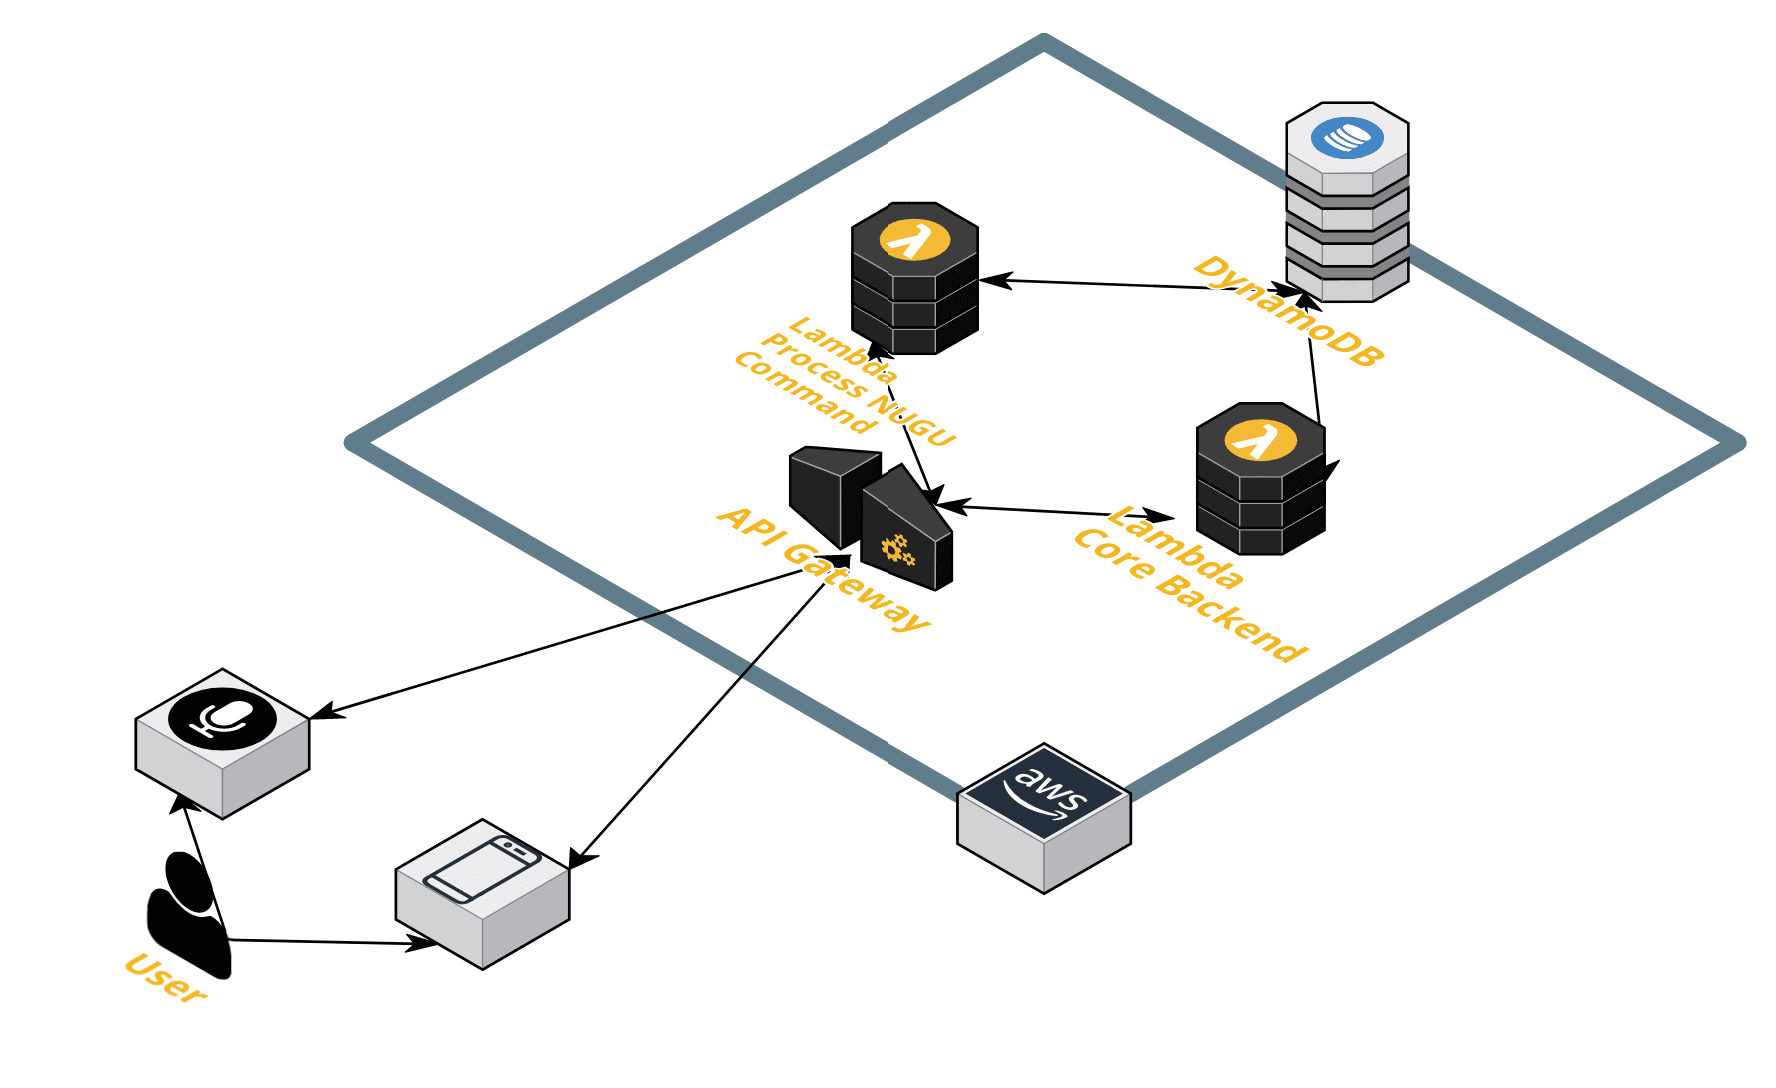
\includegraphics[width=450pt]{cloud-architecture.jpg} \caption{Overall architecture} \label{fig:Overall architecture} \end{figure} \twocolumn

\subsection{Client directory organization (React Native)} 

Our core backend service operates on AWS. Especially, serverless services such as DynamoDB and Lambda of AWS were mainly used. Client application (React Native application) request data from core backend server in Lambda. Core backend service handles requests interacting with the DynamoDB. \\
NUGU AI speaker also can make requests through other proxy server. Proxy server process the command
string which is from NUGU.

\begin{enumerate}
    \begin{table}[h]
\begin{center}
\begin{tabular}{ | m{2cm} | m{6cm} | }
\hline
\textbf{\textit{Directory}}& \textbf{\textit{Description}} \\
\hline
src/@types & It contains custom typescript type definitions. \\
\hline\
src/assets & It contains images. \\
\hline
src/components & This directory contains the smallest redundant units of components within the application. For example, StyledText components is react native css styled text component. This component is available for all components requiring Text Component. \\
\hline
src/constants & It contains constant values which are not change in application, and it is used in many situations. for example, color value like #FFFFFF is used in dark mode text color. src/constants/colors.ts file must have export const TEXT\_COLOR = '#FFFFFF'. \\
\hline
src/containers & Containers are units capable of independent functions. Having independent functions means that when a container is used, the function operates without any special conditions. Generally, several components in src/components are combined to form a container. For example, src/containers/Ranking containers that show records of the previous day include network I/O and even list up when data is received from the server. \\
\hline
src/context & Context is React api which allows subcomponents to share specific values. this directory contains custom context like GlobalTheme which is provide theme for every component. \\
\hline
src/hocs & hoc stands for High Ordered Component. Which is a design pattern used in react system. Like decorator, when a component passed through the hoc, it mounts an additional function or UX/UI. For example, with withMargin, components that pass the function (withMargin) receive a specific Margin. \\
\hline
src/hooks & hook is api which let functional component use state and other React features without writing a class. React provides some basically hooks such as useState, useEffect, but you can create custom hooks that manage your own behavior or state. It contains custom hooks made like this in this directory. for example, useTheme provides global theme value. \\
\hline
src/navigations & In React Native system, screen should be divided by bottom tab, or stacked (push means get new screen, pop means go back to before screen). reactnavigation is a opensource for these actions. this directory contains navigation definitions. \\
\hline
src/redux/modules & Redux is predictable state container. It manages application state globally. Centralizing application's state and logic enables powerful capabilities like undo/redo, state persistence, and much more. And each module is a part of redux store. for example, auth module manages access token for authentication. record manages dashboard logs. \\
\hline
src/screens & Screens are the biggest UI component. It means literally one screen. The screen consists of multiple Contenders or Components, and is connected to Navigation. \\
\hline
src/utils & Utils directory contains functions which are reusable in many context. for example, time.ts util file has functions related with dealing with date or time. \\
\hline
\end{tabular}
\label{tab1}
\end{center}
\end{table}

\item Container, component and screen modules \\
    Container, component and screen modules are UI related modules. These modules draw screen and show some data to users. In this case, the module should do two things. First is to draw default layout UI like button, scroll view for list and text input box. Second is to process data, which is used in that UI, like onClickButton function, fetching rank (data list) from server and updating new date. The source code of the application was separated according to these two concerns. Presenter.tsx focuses on drawing the UI shown (First concern). And the tsx file, identical to the module name, concentrates on processing the data (Second concern). For example, src/screens/Setting and src/containers/Ranking module directories look like: \\
    
    \begin{lstlisting}[frame=single]
    src/
        ...
        containers/
            Ranking/
                index.tsx
                Presenter.tsx
                Ranking.tsx
        ...
        screens/
            Setting/
                index.tsx
                Presenter.tsx
                Setting.tsx
        ...
    \end{lstlisting}
    
    Setting.tsx and Ranking.tsx concentrate on processing data. Both of Presenter.tsx focus on UI. \\ 
    Exceptionally, if a module has little to process data, there is no Presenter.tsx, and UI drawing is handled in a [module name].tsx file. \\
    
\item HOC, Hook \\
    HOC, hook has special naming convension. HOC name should start with "with" and hook name must start with "use". withController.ts, withPadding.ts and withStyledViewLayout.ts are in src/hocs. useCurrentTask.ts, useEditableState.ts, and useTheme.ts are in src/hooks.
    
\end{enumerate}
    \subsection{Backend directory organization} \\
    \begin{enumerate}
    \begin{table}[h]
\begin{center}
\begin{tabular}{ | m{1cm} | m{7cm} | }
\hline
\textbf{\textit{Directory}}& \textbf{\textit{Description}} \\
\hline
cmd & In cmd, the modules are divided according to the environment in which the serverruns. There are api, dev, local modules. api module is forlambda environment (for production deploy). dev module is for ubuntu development server. And local module is for local development. \\
\hline\
internal & Private application and library code. This is the code developer don't want others importing in their applications or libraries. Note that this layout pattern is enforced by the Go language compiler itself. Main source codes for application are in this directory. cmd doesn't have many code. Modules in cmd should import features from internal. \\
\hline
scripts & Scripts to perform various build, install, analysis, etc operations. Our scripts directory has a few database initiating script. \\
\hline
\end{tabular}
\label{tab1}
\end{center}
\end{table}

    \item The internal Modules \\
The internal directory contains modules in functional units. For example, user modules, which are modules responsible for user-related functions, such as changing user information or leaving, exist in the internal directory. And one feature modules consists basically of three things, module.go, controller.go, and service.go. So, user module directory consists of user.module.go, user.controller.go, and user.service.go. \\ 
    
    \begin{lstlisting}[frame=single]
    internal/
        user/
            user.module.go
            user.controller.go
            user.service.go
            ...
    \end{lstlisting}
    
    module.go acts as a connection point to connect the module to the server. module.go initiates controller.go which is router. And controller.go. The controller.go uses service.go to process several detailed service logic interacting with a database, etc. \\
    There may be additional files like struct.go or validation.go. structure.go defines Data Transform Object (DTO) coming from clients. And validation.go is used when additional verification is required in addition to the verification process, which is basically filtered by go-gin. \\
    
\item The internal/shared Module \\
Unlike modules in common functional units, shared modules contain codes commonly used in modules in all functional units. The shared module looks like below. \\
    
    \begin{lstlisting}[frame=single]
    internal/
    ...
        shared/
            configs/
                configs.go
            database/
                schema/
                    profile.schema.go
                    record.schema.go
                    ...
                query.go
                database.go
            middlewares/
                authMiddleware.go
            types/
                ...
            utils/
                ...
    \end{lstlisting}
        \begin{enumerate}
            \item configs: configs module sets OS environment to string and provides it.
            \item database: There is a schema form, and a code for queries.
            \item middlewares: The code that serves to process the request before entering the controller is contained.
            \item types: The transform code or processing code associated with the data type is included.
            \item utils: This module contains the util functions used in many places. \\
        \end{enumerate}
    \end{enumerate}
            
\subsection{Proxy server directory organization} \\ 
In STMT, NUGU AI speaker sends requests to Proxy Server. Proxy Server communicates with STMT Server to respond appropriately to speaker's requests and then responds with organized information in the form required by NUGU AI speakers. In this process, Proxy Server sometimes invokes two or more APIs for a single request. Proxy Server is written in django and follows default structure of django.\\

\begin{enumerate}
    \begin{table}[h]
    \begin{center}
    \begin{tabular}{ | m{3cm} | m{5cm} | }
    \hline
    \textbf{\textit{Directory}}& \textbf{\textit{Description}} \\
    \hline
    nugu\_proxy & The project directory across the proxy server. It consists of app directories such as app/, nugu\_proxy/ and setup files such as .gitignore, requirement.txt, and zappa\_settings.json. manage.py also exist here. \\
    \hline\
    nugu\_proxy/nugu\_proxy & The part that manages the entire project. Here are the setting files for the whole project and the files responsible for the first url routing. \\
    \hline
    nugu\_proxy/app & The part related to the actual service logic. The url pattern and functions to be executed on url request are defined here. \\
    \hline
    \end{tabular}
    \label{tab1}
    \end{center}
    \end{table}

The overall structure of proxy server is as follows: \\ \\

    \begin{lstlisting}[frame=single]
    nugu_proxy/
        app/
            __init__.py
            apps.py
            urls.py
            views.py
            
        nugu_proxy/
            __init__.py
            settings.py
            urls.py
            wsgi.py
	
	.env
	.gitignore
	manage.py
	requirement.txt
	zappa_setting.json
    \end{lstlisting}
    
        \item urls.py
            \begin{lstlisting}[frame=single]
# nugu_proxy/nugu_proxy/urls.py

from django.contrib import admin
from django.urls import path, include

urlpatterns = [
    path('admin/', admin.site.urls),
    path('', include('app.urls'))
]
            \end{lstlisting}
            \begin{lstlisting}[frame=single]
#nugu_proxy/app/urls.py

from django.urls import path
from app import views

urlpatterns = [
    path('response.task_list', 
    views.task_list),
    path('complete_task', 
    views.complete_task),
		...
            \end{lstlisting}
            If requested url is defined, execute view function. The proxy server verifies that the request is url as defined in nugu.proxy/nugu.proxy/urls.py. Requests other than '{{ host }}/admin/' are verified including the patterns defined in app/urls.py. \\ \\
            
        \item views.py: \\
        The part where the service logic is defined. django has a pattern structure called MTV, which is the same as the MVC pattern structure. MTV means Model, Template, and View. Template corresponds to View in MVC pattern and View to Controller in MVC pattern. The function corresponding to View is defined in views.py. The defined function is executed when the url request is matched. The view function returns the response in json format after the required work is done for each request. \\ \\
        
        \item .env, manage.py: \\
        Sensitive information such as AWS\_ACCESS\_KEY is separated into an .env file and used as an environmental variable. Environmental variables are read in manage.py. \\ \\ \\ \\ \\ \\ \\ \\
            \begin{lstlisting}[frame=single]
# manage.py

import os
import sys
import dotenv

if __name__ == '__main__':
    dotenv.read_dotenv()
    os.environ.setdefault(
    'DJANGO_SETTINGS_MODULE', 
    'nugu_proxy.settings')
    try:
        ...
            \end{lstlisting}
        
        \item .gitignore: \\
        This file specifies the files and folders to ignore in the git. This can be used to prevent the mistake of releasing files such as .env. \\
        \item requirement.txt: \\
        A list of packages used by proxy servers. \\
        \item zappa\_setting.json: \\
        Settings are defined for deploy with zappa at aws lambda. \\
            
    \end{enumerate}
    

\section{Use Cases}
\subsection{Use case 1 Login:} 

User can login through their Google account. If the user is already logged in, the screen will show the main page immediately.

\begin{enumerate}

\begin{figure}[h] \centering 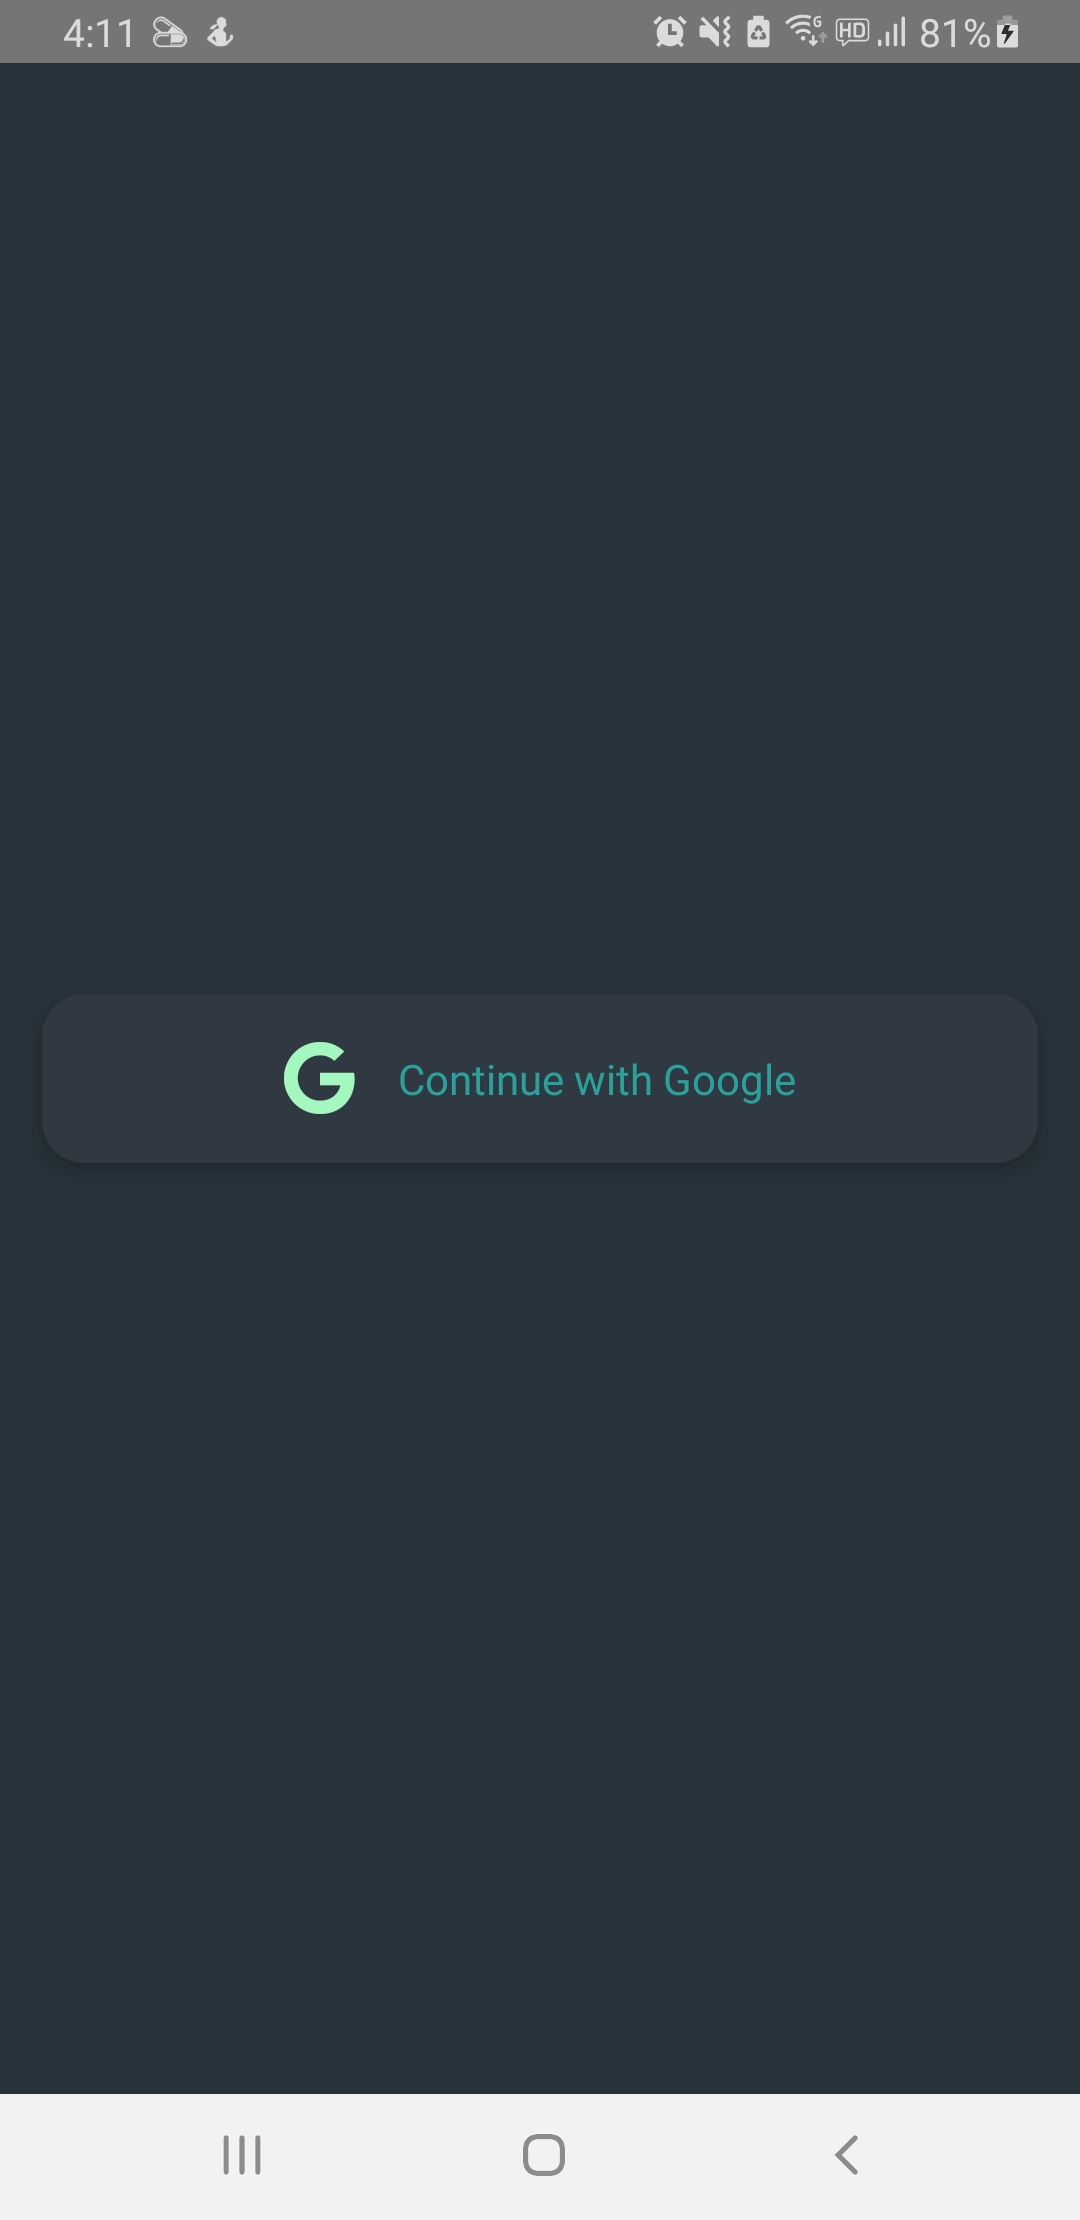
\includegraphics[width=200pt]{Google Login.jpg} \caption{Login Screen} \label{fig:Login Screen} \end{figure} 

    \item Login screen is the first screen that users can see when they are not logged in to our application. The login button will lead the users to the google login service, and our server will receive their information from google.
\end{enumerate}

\subsection{Use case 2 Main Screen:}

\begin{figure}[h] \centering 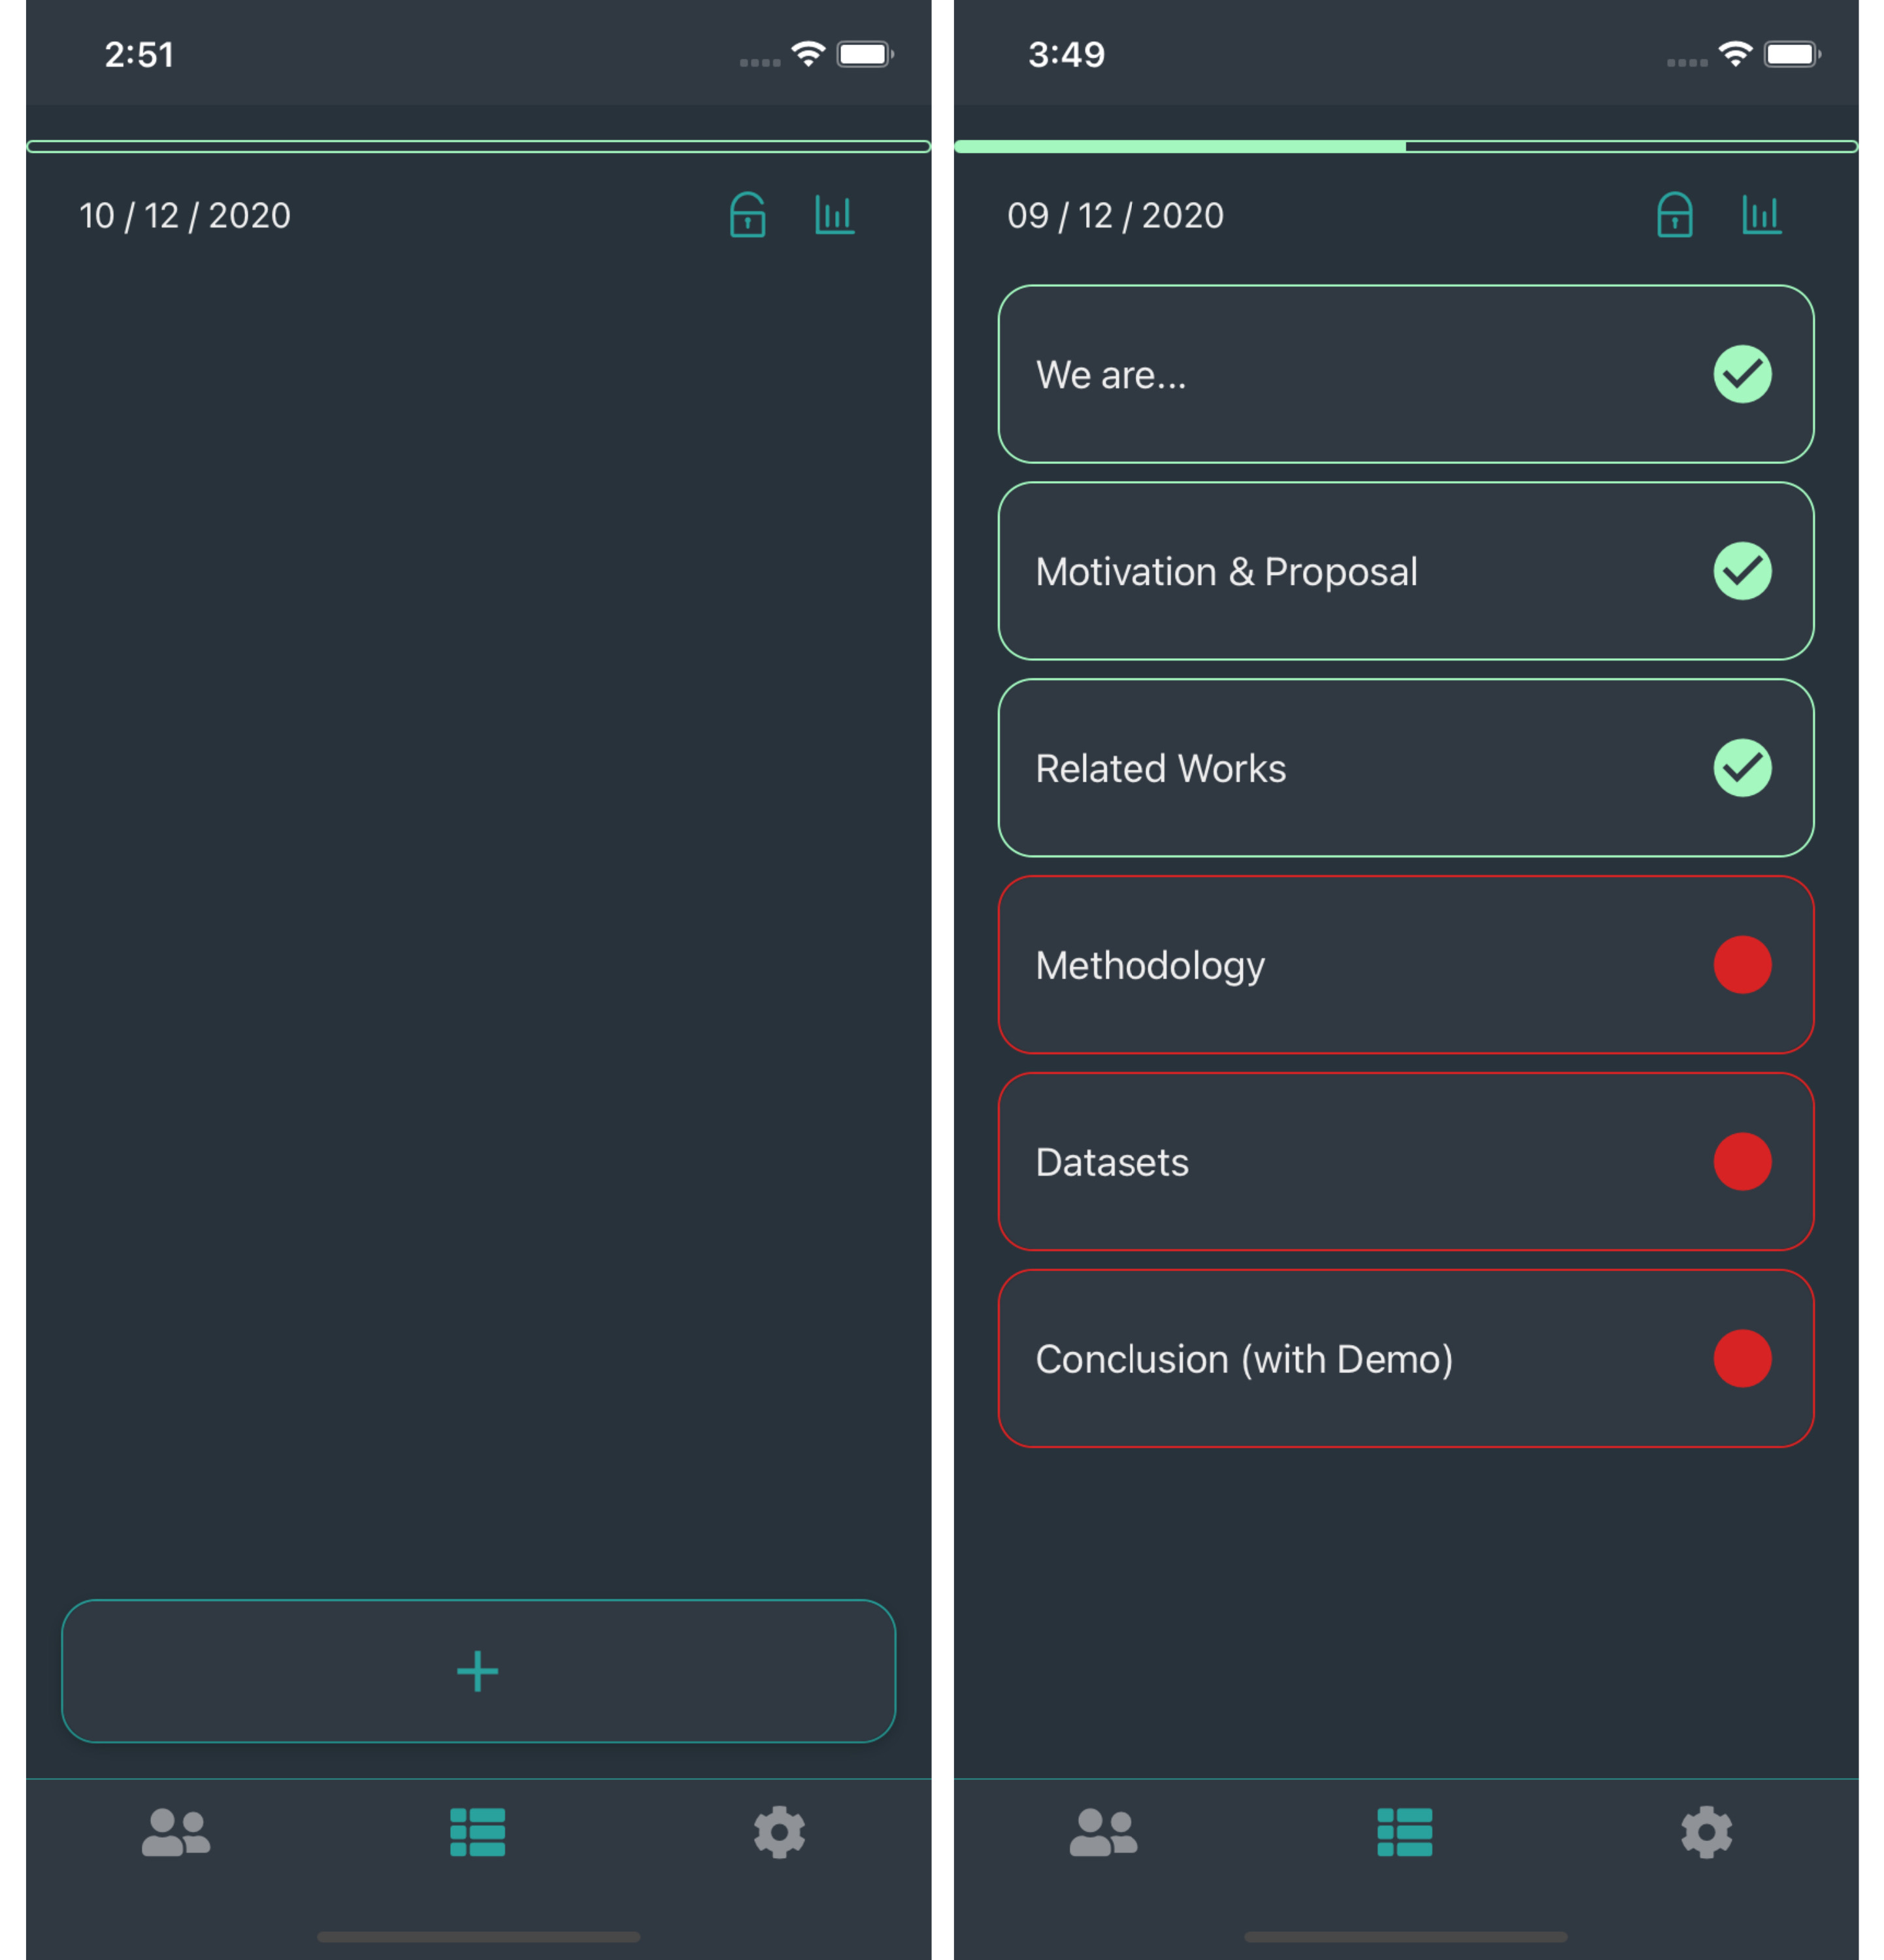
\includegraphics[width=270pt]{Main Screen최종.jpg} \caption{Main screen} \label{fig:Main Screen} \end{figure}

Progress bar is on the top of the main screen. The colored part is the percentage of the tasks that is done by the user each day. Task lock and dashboard buttons are on the right and add button will be the only thing that users can click, if users did not set any tasks. Add button will disappear when users set six tasks, which is the maximum. They can make tasks by the add button and set specific details.

\begin{enumerate}

\begin{figure}[htp] \centering 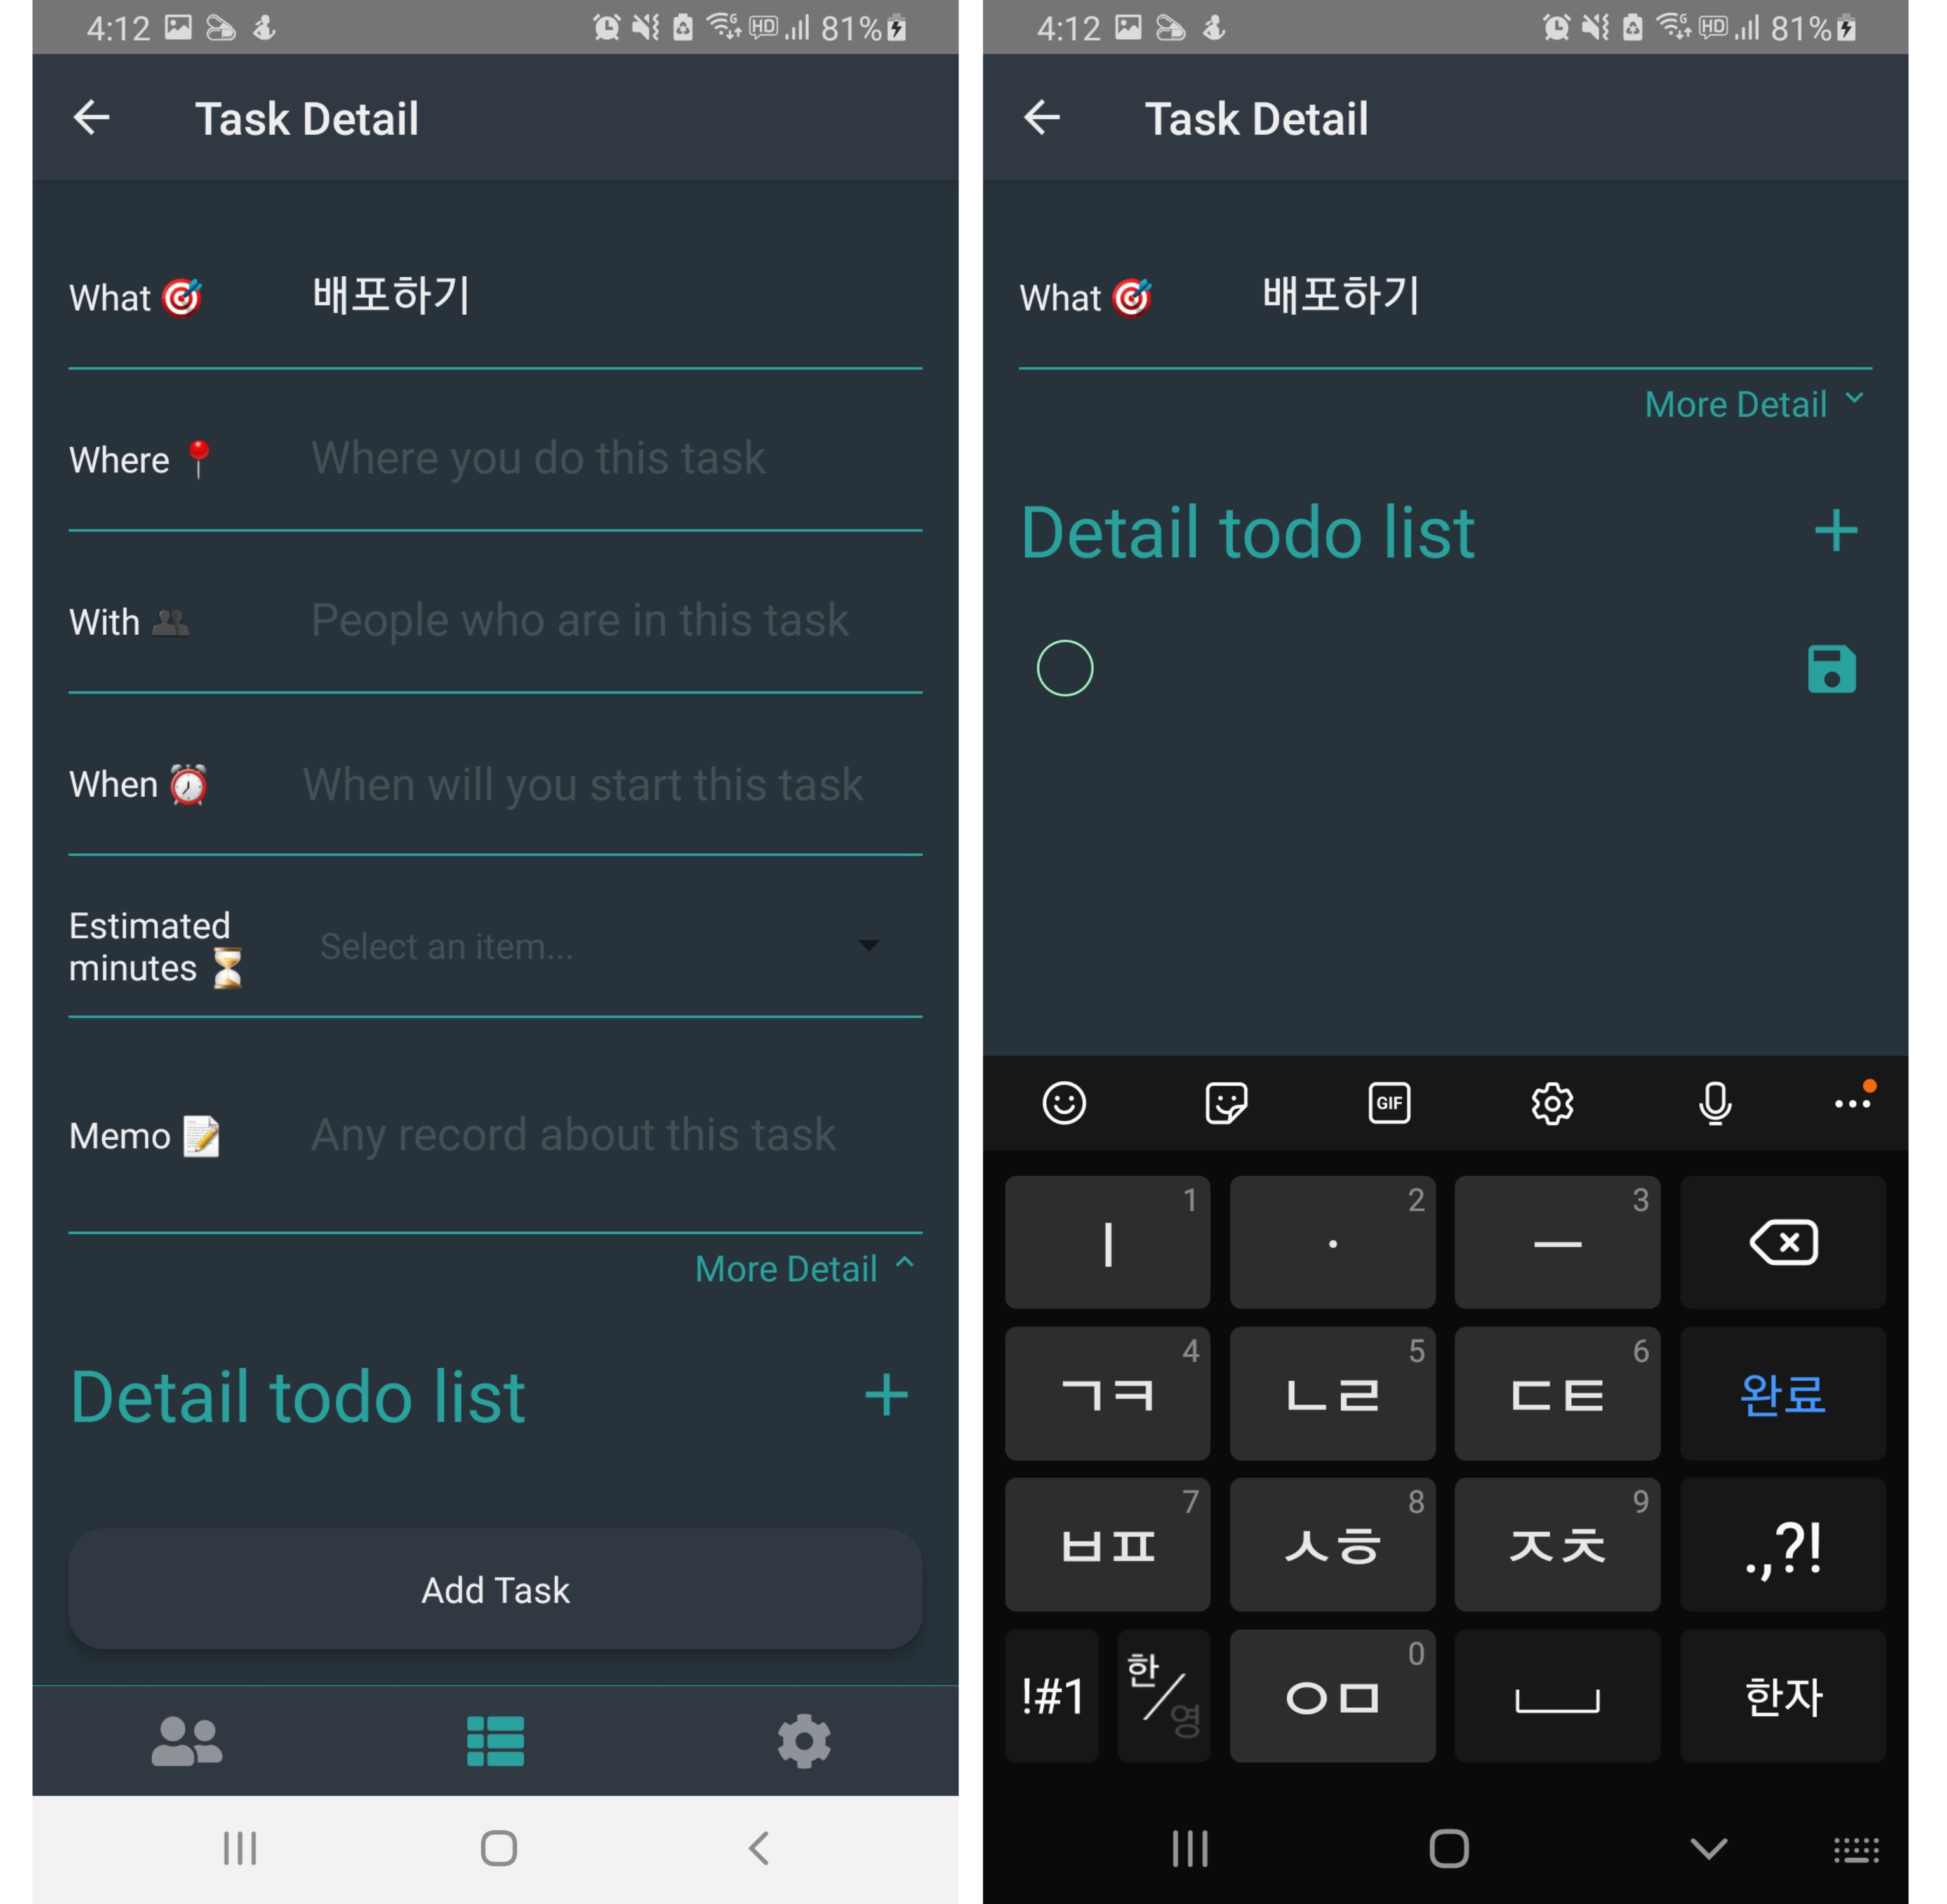
\includegraphics[width=270pt]{Task Detail최종.jpg} \caption{Setting task details} \label{fig:Task Detail} \end{figure} 

    \item When the user clicks the add button or the task itself, the screen will turn into specific tasks screen. Users can set the starting time, set the place where the task is going to be executed, and make detailed notes to each task. To-do list is also included in each task so that users can set a more detailed task.
    
\begin{figure}[htp] \centering 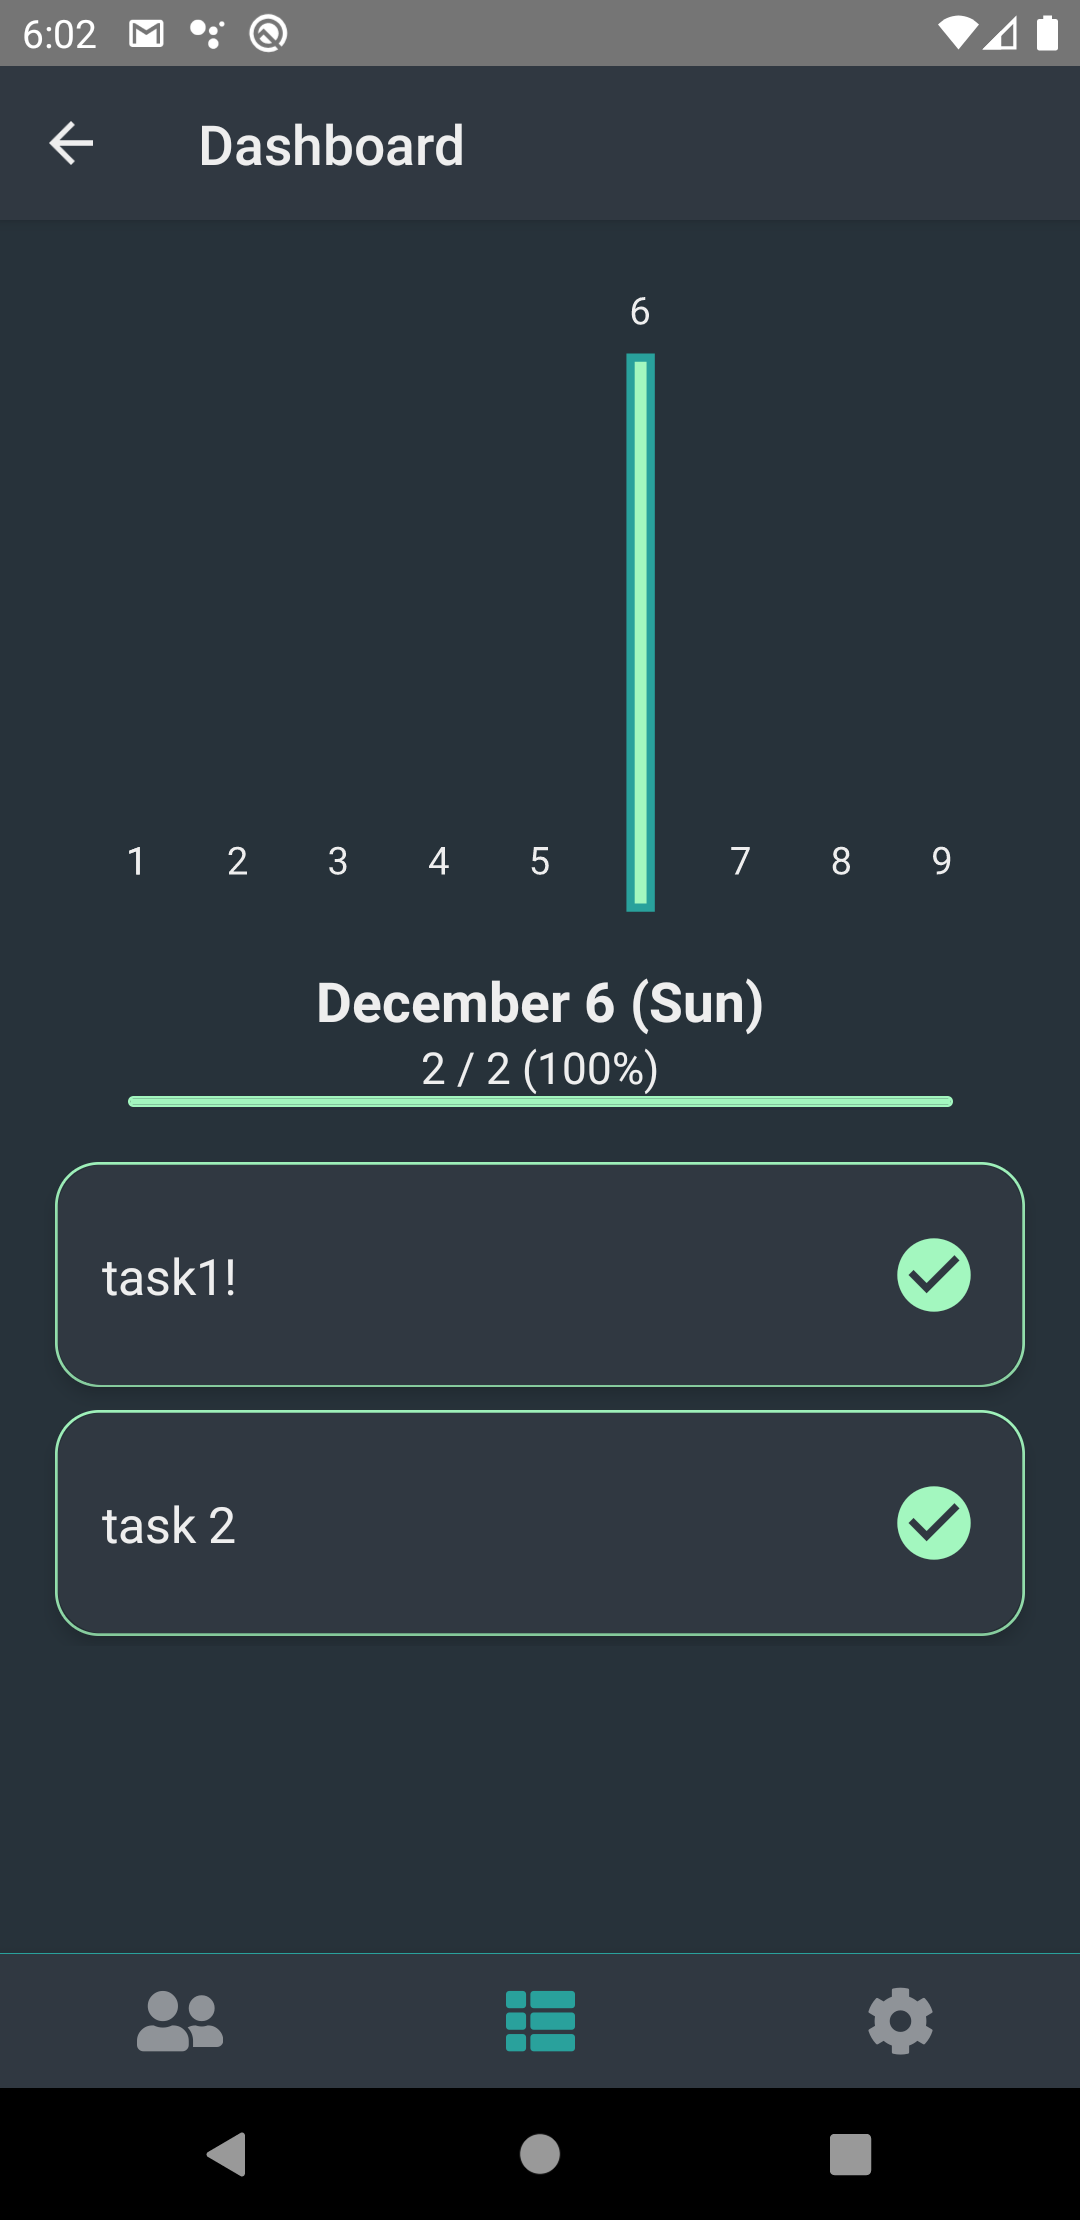
\includegraphics[width=200pt]{Dashboard최종.png} \caption{Dashboard} \label{fig:Dashboard} \end{figure}    
    
    \item Dashboard shows the result of finishing the task in a bar graph. By clicking the graph or the day itself, they can select a date to view the results of the day, and the previous list of six tasks will be shown to the users. Previous tasks are viewed exactly like the tasks on the main screen.

\end{enumerate}

\subsection{Use case 3 Social:}

\begin{figure}[htp] \centering 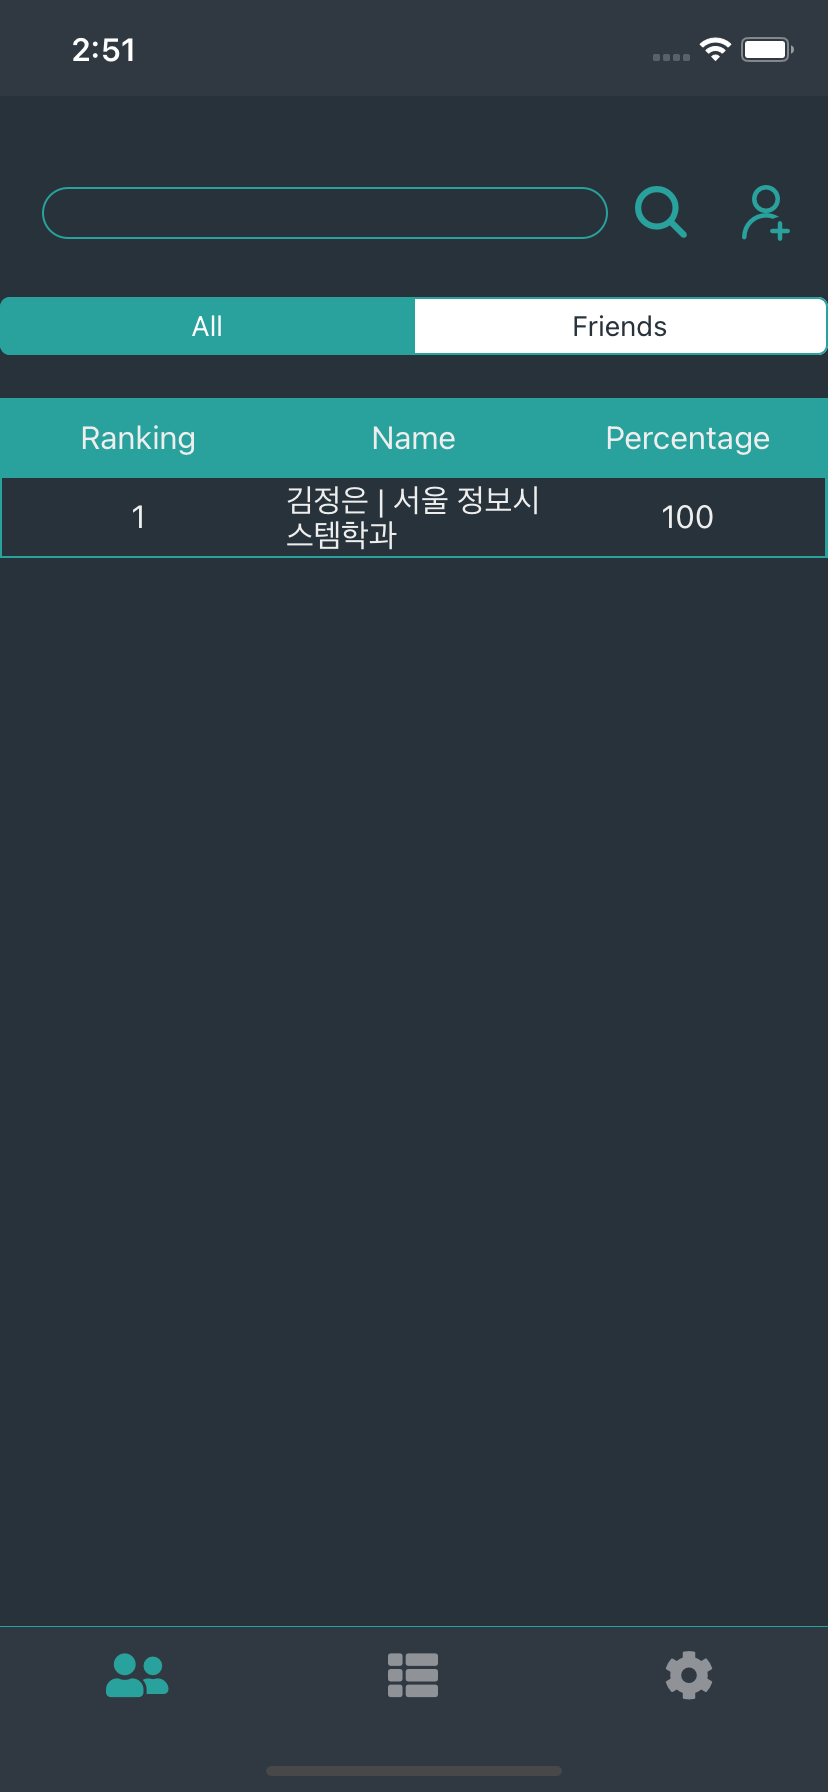
\includegraphics[width=200pt]{Social Screen최종.png} \caption{Social Screen} \label{fig:Social Screen} \end{figure}

In the social screen, there is a bar where users can search for their friend's name and their task results, and an add button to add friends using google email. When users press the tab, they can take turns looking at the list of their friends or the list of other users who use this application, so the list looks different depending on the tab. Users can also share their results externally with the share button.

\begin{enumerate}

    \item Users can search their friends by typing the name of their friends in the bar. Then the screen will show the list of the name that users have entered.
    
    \begin{figure}[htp] \centering 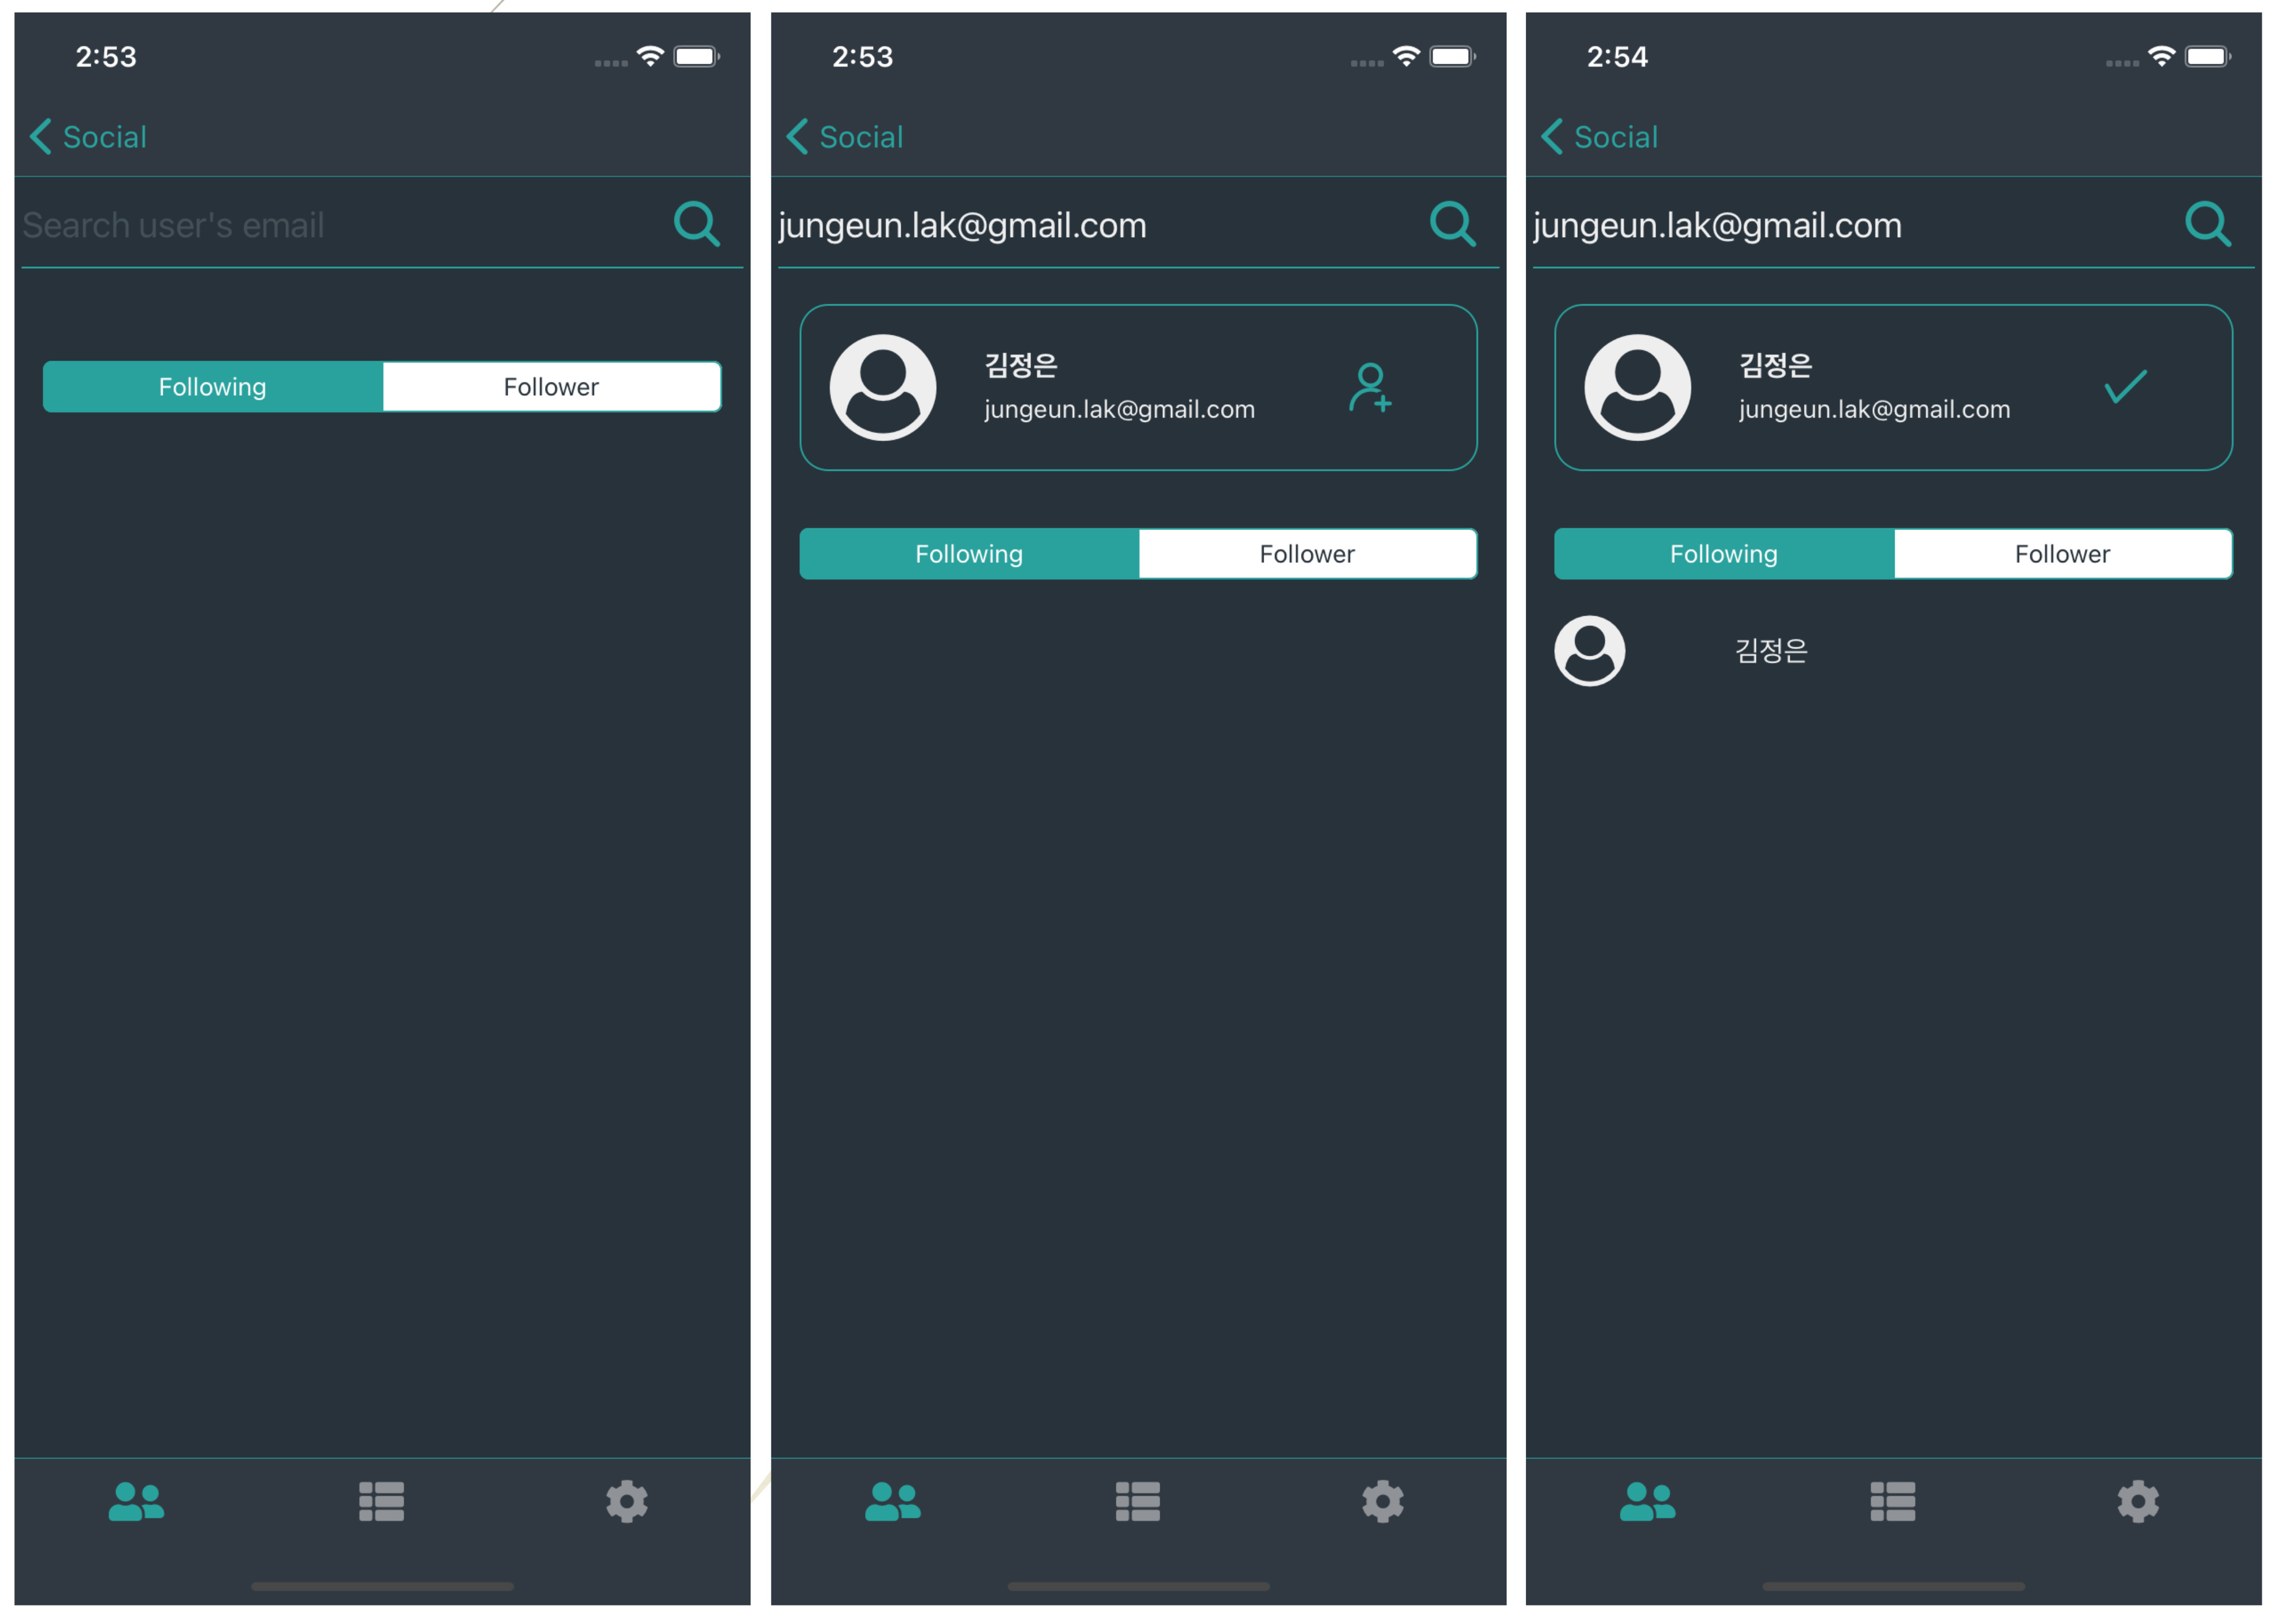
\includegraphics[width=260pt]{Add Friends최종.jpg} \caption{Add friends} \label{fig:AddFriends} \end{figure} 
    
    \item Add icon on the right side of the bar is a button that can add friends to the friends list. When the button is clicked, the screen will turn into Search user screen. User can enter friend's google e-mail address to add to a friend list. However, if the user enters an e-mail address that does not exist, nothing comes up. Following and follower are shown through this screen.
    \item Tab is divided into two categories: Friends, All  . Users can press friends tab to see the list of friends or press all tab to see the ranking of all the users who are using our application.
    \item The list gives three information: rank, name, and percentage(score). Users can see the ranking by comparing themselves to the others. Percentage is for the ranking and is the sum of the percentage that users have completed the task. If there are users with the same score, they just go in order.
    \item Share button at the bottom of the list is a feature that allows users to share their results externally. If they press the button, they can choose where to share, and then the ranking screen will be shared as a photo.
\end{enumerate}

\begin{figure}[htp] \centering 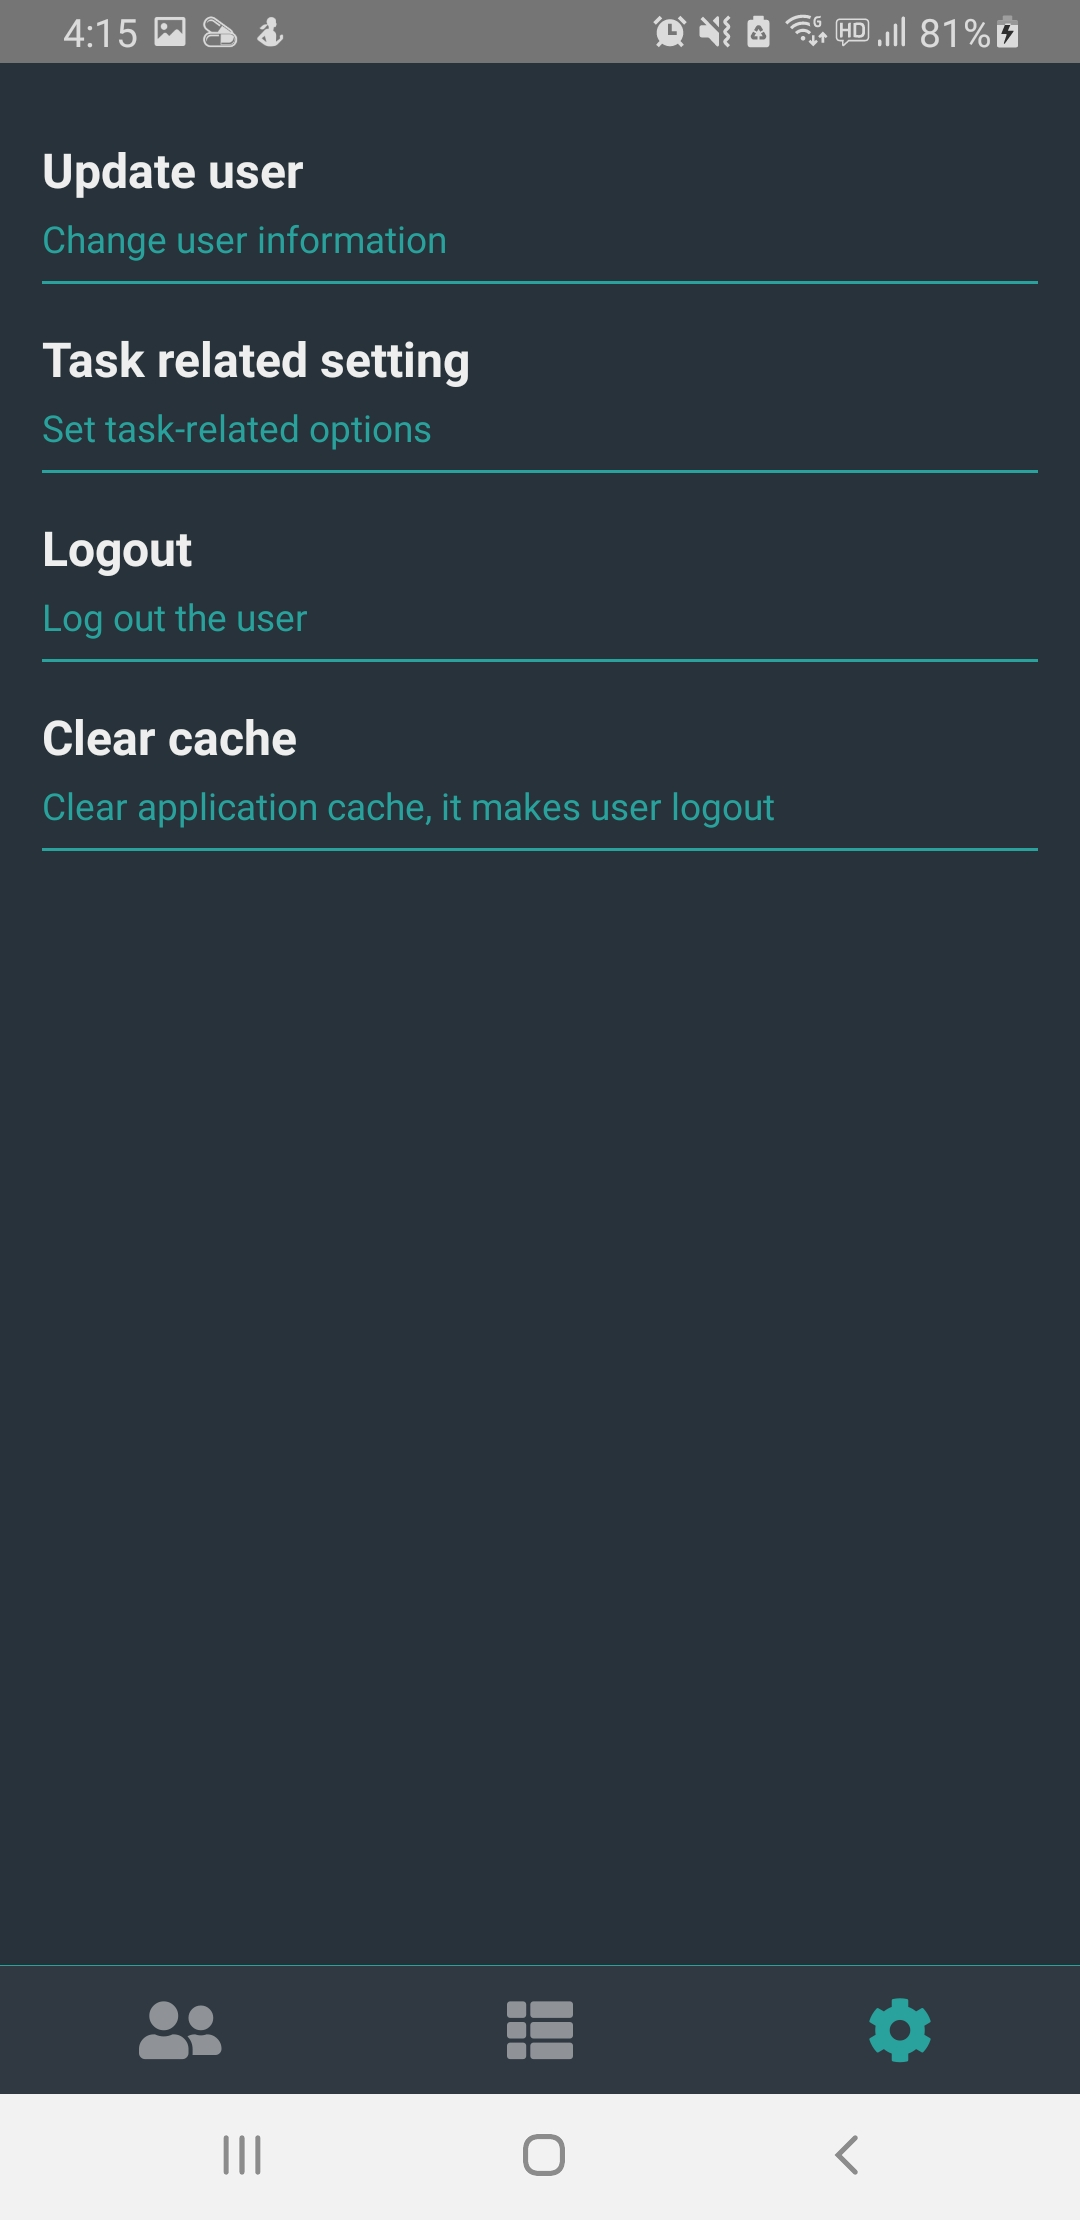
\includegraphics[width=200pt]{Settings.jpg} \caption{Settings} \label{fig:Settings} \end{figure}

\subsection{Use case 4 Settings:}
There are four features in Settings Screen: Update user, Task related setting, Logout, and Clear cache.

\begin{enumerate}

\begin{figure}[htp] \centering 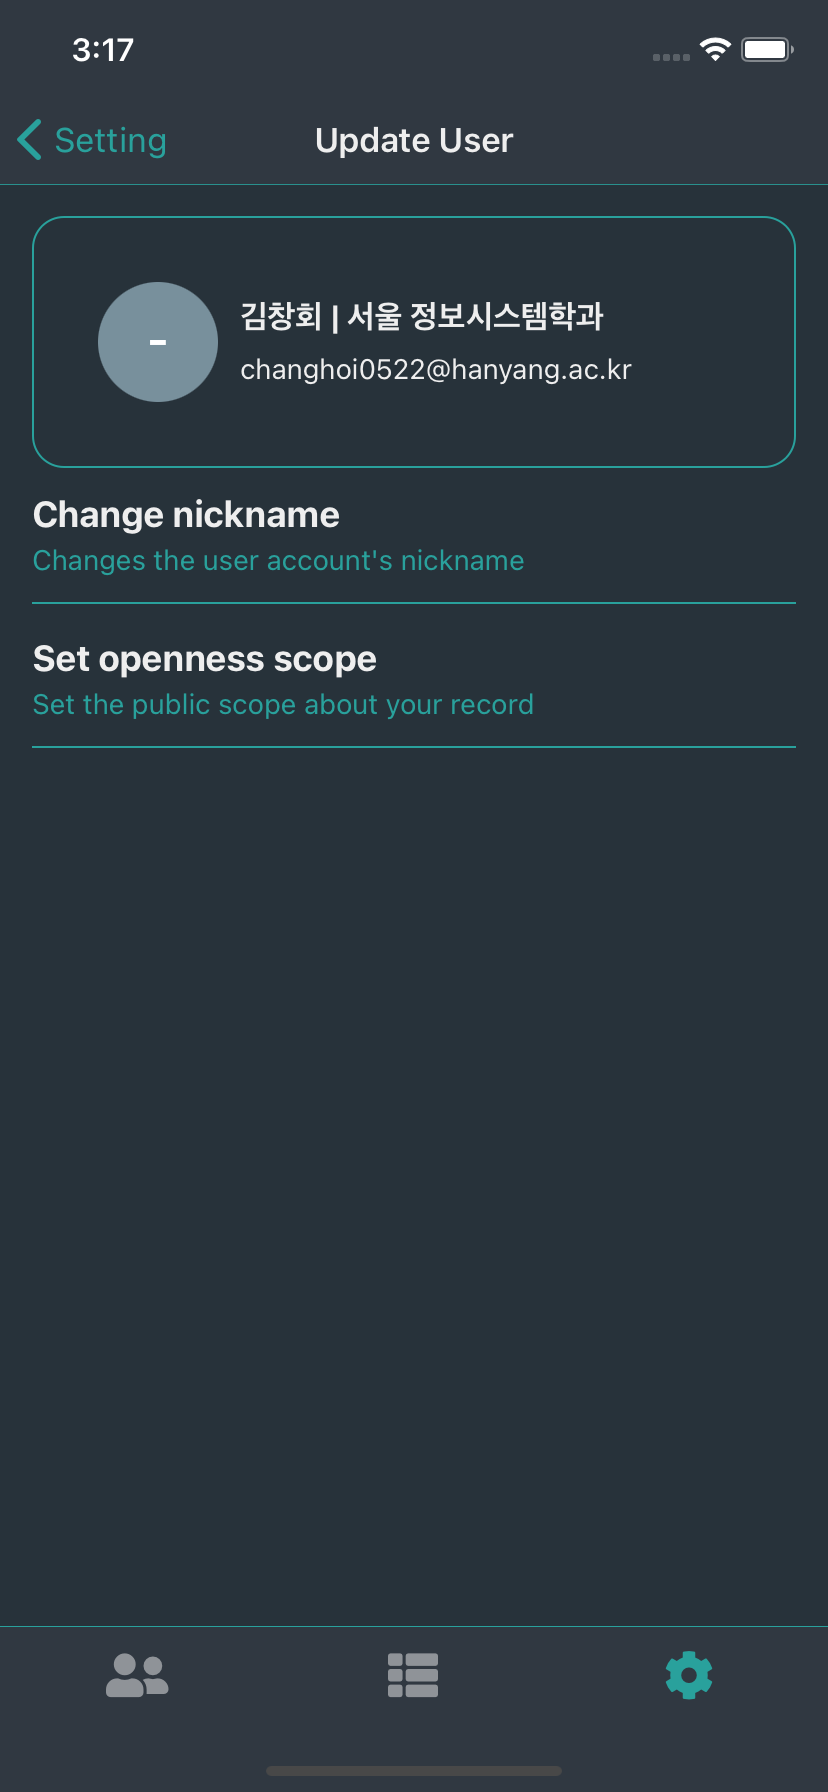
\includegraphics[width=200pt]{Update User최종.png} \caption{Update User} \label{fig:Settings} \end{figure}

    \item Users can modify their nickname by pressing Update user. In addition, they can set whether they want to expose their records or not. Users can make three choices: 1. Show their records to everyone. 2. Show their records only to their friends. 3. Don't expose their records at all. Depending on the user, their records may or may not be seen by others.
    
    \begin{figure}[htp] \centering 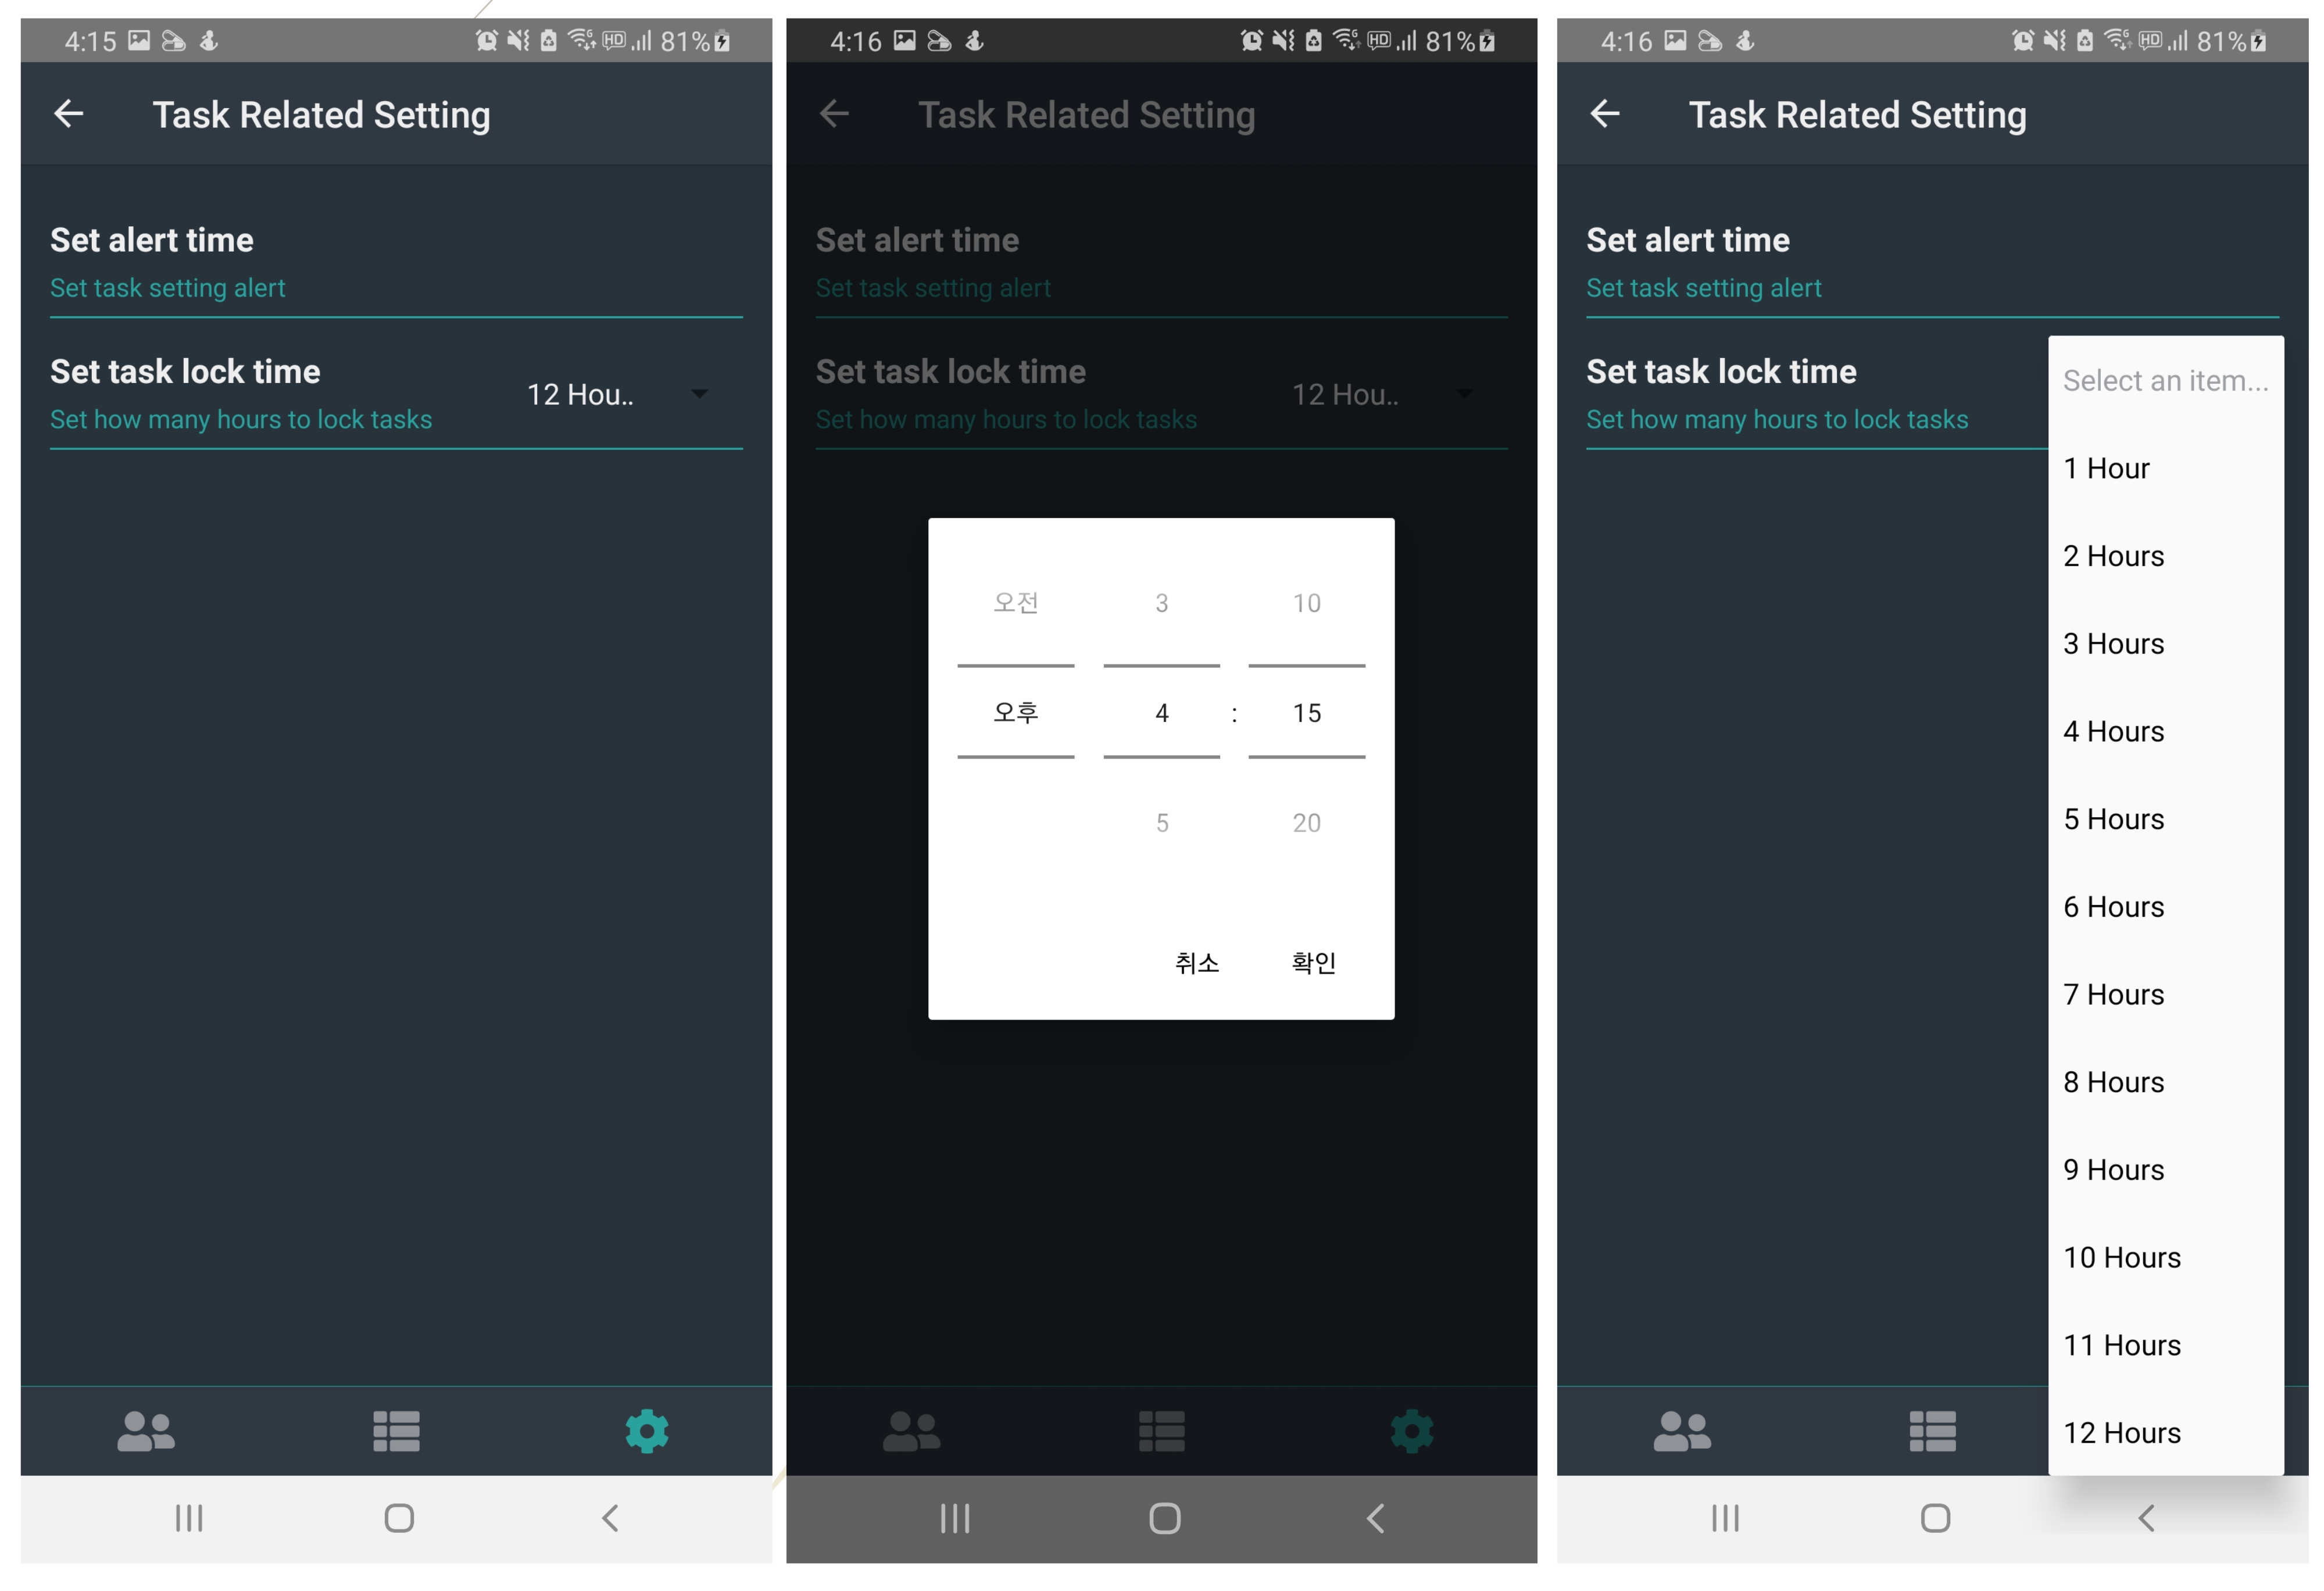
\includegraphics[width=260pt]{Task Related Setting최종.jpg} \caption{Task Related Setting} \label{fig:Settings} \end{figure}
    
    \item Task related setting can set the alert time and the task lock time. When the user set the alert time, the alarm will ring at that specific time every day. This gives users who have forgotten to work on their tasks a chance to remind them once more. If task lock time setting is set by the user and then the task is locked, the user cannot modify the task during the locked time, and the daily record will be stored based on the task lock time, which is used to score users in the list of social screens.
    
    \item Logout makes user log out the application. Clear cache does the same thing, but at the same time, clears application cache.
    
\end{enumerate}

\section{Installation Guide}
\subsection{Before GA (General Availability} 
\begin{enumerate}

    \item Setup React native development environment. (https://reactnative.dev/docs/environmentsetup)
    \item Clone application git repository \\
    git clone https://github.com/6-things-must-to-do/app.git
    \begin{enumerate}
        \item Check .env file in root directory of code base. It should have STAGE value, and production.
    \end{enumerate}
    \item Create Google Firebase project for authentication. (https://console.firebase.google.com). Both iOS and Android application package's name must be com.stmt. Then, download google-services.json for android and GoogleService-Info.plist for iOS.
    \begin{enumerate}
        \item Check google-services.json file in android/app/.
        \item Check GoogleService-Info.plist file in ios/STMT/.
    \end{enumerate}
    \item In code base directory, install packages for application (Make sure that yarn is available - npm i -g yarn ) \\
    cd app \&\& yarn
    \item (Only for iOS build) Install Cocoapod packages. \\
    cd ios \&\& pod install
    \item After all above stage, you can build application in both iOS and Android.
    \begin{enumerate}
        \item iOS: yarn ios
        \item android: yarn android
    \end{enumerate}
    CAUTION: In old version of Android OS, application might be unavailable.
\end{enumerate}

\subsection{After GA}
Just download the application from the App Store.
\end{document}